%%%%%%%%%%%%%%%%%%%%%%%%%%%%%%%%%%%%%%%%%%%%%%%%%%%%%%%%%
%%%
%%%  第4章
%%%  参考文献の表示
%%%
%%%%%%%%%%%%%%%%%%%%%%%%%%%%%%%%%%%%%%%%%%%%%%%%%%%%%%%%%
% \section{Locomotion \& Motion Selection}
This section drives into the locomotion strategy for Moonbot with full configuration operation. The motion control is orchestrated through the integration of ROS2 control framework. The joint trajectory controller is used to operate the multiple joints.

\section{Joint Trajectory Controller}
ROS2 control offers a versatile tool called \texttt{ros2\_controllers} \cite{ros2controllers}, designed as a controller interface accommodating various robot specifications. For example, the \texttt{position\_controller} can accept position inputs and generate corresponding outputs to a position interface. Similarly, the \texttt{velocity\_controller} receives input and produces velocity output. Additionally, specialized controllers like the \texttt{diff\_drive\_controller} provide advanced control interfaces tailored for mobile robots equipped with wheeled locomotion systems.

For precise control of Moonbot's dynamic locomotion, the \texttt{joint\_trajectory\_controller} from ROS2 is utilized. This controller executes joint-space trajectories on multiple joints, enabling smooth and dynamic locomotion by interpolating the waypoints to desired target at specific time. 

There are three strategies for spline interpolation, depending on specification of those waypoints. 

\label{itemize jtc}
\begin{itemize}
    \item Linear: Only position is specified so it provide the continuity of joint trajectory only at the position level. 

    % \begin{figure}[h]
    %   \centering
    %   \includegraphics[width=130mm]{./fig/ros2_control/spline_position.png}
    %   \vspace{2mm}
    %   \caption{Joint-space trajectory for linear spline}\label{linear int}
    % \end{figure}

    \item Cubic: Position and velocity are specified so the continuity is confirmed at the velocity level.

    % \begin{figure}[h]
    %   \centering
    %   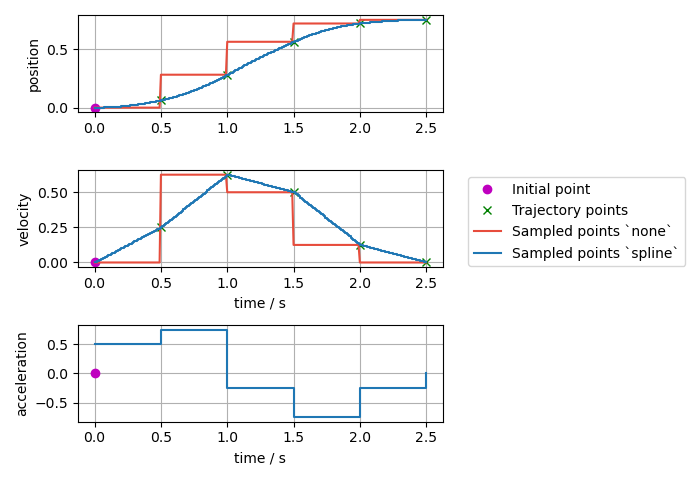
\includegraphics[width=130mm]{./fig/ros2_control/spline_position_velocity.png}
    %   \vspace{2mm}
    %   \caption{Joint-space trajectory for linear spline}\label{cubic int}
    % \end{figure}

    \item Quintic: Position, velocity and acceleration are specified: Guarantees continuity at the acceleration level.

    % \begin{figure}[h]
    %   \centering
    %   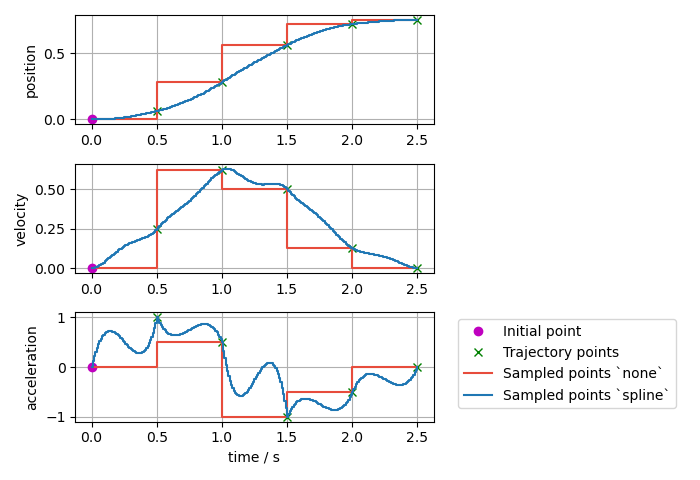
\includegraphics[width=130mm]{./fig/ros2_control/spline_position_velocity_acceleration.png}
    %   \vspace{2mm}
    %   \caption{Joint-space trajectory for linear spline}\label{quintic int}
    % \end{figure}
\end{itemize}

\begin{figure}[t]
 \begin{subfigure}{1.0\textwidth}
 \begin{center}
  \includegraphics[height=80mm]{./fig/ros2_control/jtc/spline_position.png}
\caption{Joint-space trajectory for linear spline.}\label{linear int}
 \end{center}
 \end{subfigure}
 
 \begin{subfigure}{0.5\textwidth}
 \begin{center}
  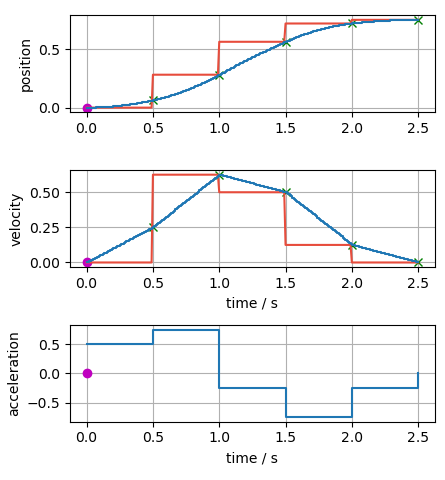
\includegraphics[height=80mm]{./fig/ros2_control/jtc/spline_position_velocity.png}
\caption{Joint-space trajectory for linear spline.}\label{cubic int}
\end{center}
\end{subfigure}
 \begin{subfigure}{0.5\textwidth}
 \begin{center}
  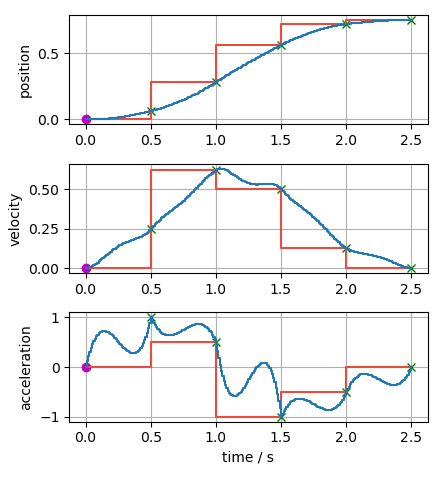
\includegraphics[height=80mm]{./fig/ros2_control/jtc/spline_position_velocity_acceleration.png}
\caption{Joint-space trajectory for linear spline.}\label{quintic int}
\label{subfig3}
 \end{center}
 \end{subfigure}
\vspace{-2mm}
\caption{Spline interpolation Strategies of joint trajectory controller.}
\label{interpolation}
\end{figure}

The joint-space trajectories for each case are illustrated in \fig{interpolation}. In this time, Moonbot is using only position linear interpolation for easier prototyping the motion control and designing gait motion.

\section{Gazebo Simulation}
Gazebo \cite{gazebo} stands as a robust open-source 3D simulation environment widely used in the robotics community. Its physics engine, sensor simulation, and realistic rendering capabilities make it a choice for testing Moonbot's motion and control strategies in both earth-based environment and lunar landscape environment.

%%%
\begin{figure}[t]
 \begin{subfigure}{0.5\textwidth}
 \begin{center}
  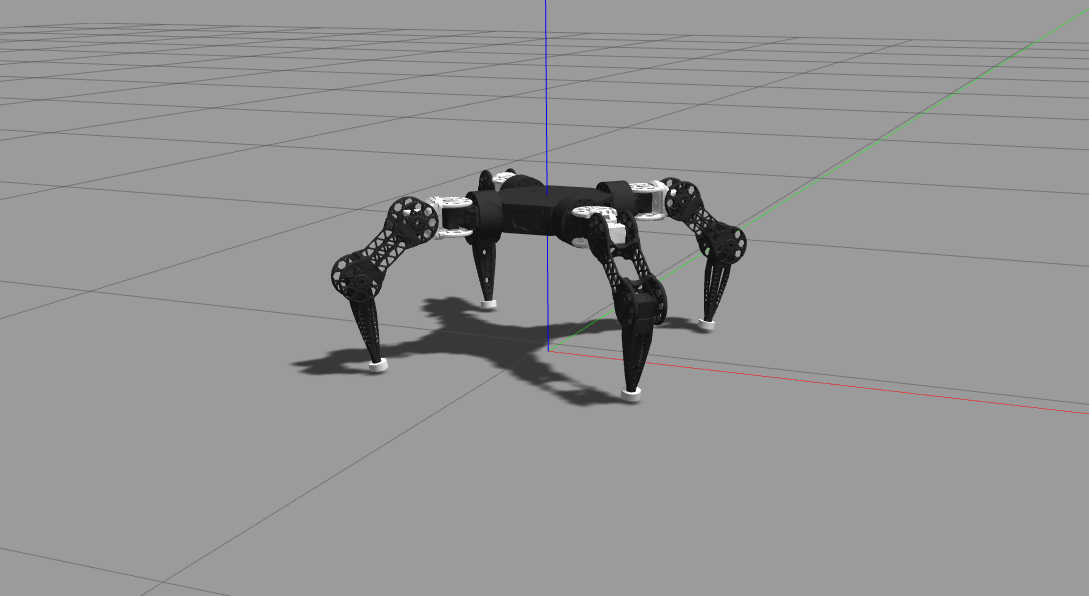
\includegraphics[width=78mm]{./fig/chap4/simulation/moonbot_gazebo.png}
\caption{Earth ground environment.}\label{subfig_gazebo1}
\end{center}
\end{subfigure}
 \begin{subfigure}{0.5\textwidth}
 \begin{center}
  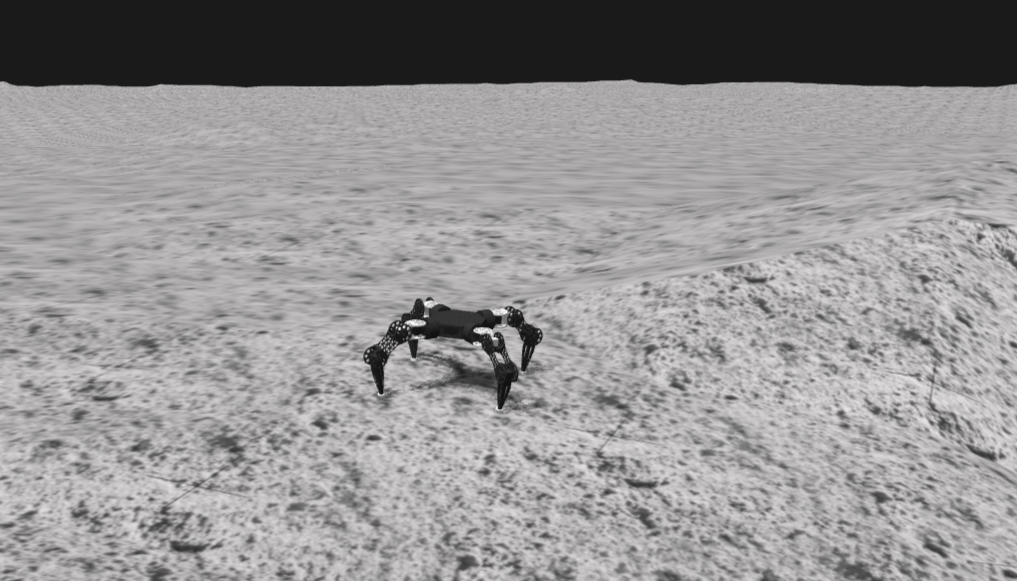
\includegraphics[width=75mm]{./fig/chap4/simulation/moonbot_gazebo5.png}
\caption{Lunar surface environment.}\label{subfig_gazebo2}
 \end{center}
 \end{subfigure}
\vspace{-2mm}
\caption{Moonbot in Gazebo simulation.}
\label{gazebosim}
\end{figure}
%%%

\section{Kinematics Model of Legs Motion}

The inverse kinematics (IK) model is used as a function for calculate the joint positions, based on the given coordinates of the end effector's position in the leg's coordinate system.

Let $(x, y, z)$ represent the desired coordinates of the end effector position in the leg's coordinate system, as shown in \fig{leg_config}. The IK algorithm calculates the joint angles $(\theta_1, \theta_2, \theta_3)$ corresponding to the coxa, femur, and tibia joints, respectively. 

The result of coxa joint $(\theta_1)$, responsible for lateral movement, is limited within a span of -90 to 90 degrees. Similarly, the femur joint $(\theta_2)$, facilitating forward and backward motion, adheres to the same range of -90 to 90 degrees. Finally the tibia joint $(\theta_3)$ spans from -100 to 100 degrees. These specified limits ensure that the leg articulates within safe and mechanically feasible parameters.

\begin{figure}[h]
  \centering
  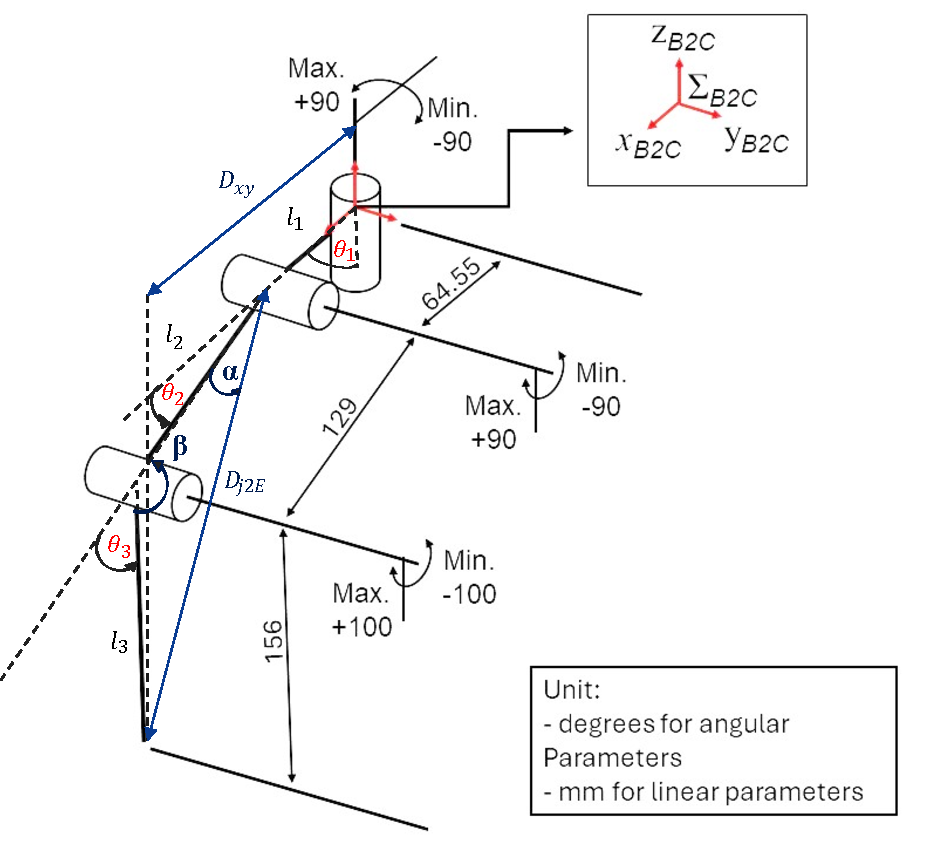
\includegraphics[width=120mm]{./fig/leg_configuration/IK.pdf}
  \vspace{2mm}
  \caption{Configuration of leg's module of Moonbot.}\label{leg_config}
\end{figure}

First, we initialize the parameters including the lengths of the leg segments ($l_1, l_2, l_3$) for coxa, femur, and tibia, respectively.

Inverse Kinematics Calculation:
    \begin{itemize}
      \item First, we calculate the distance from the coxa joint to the EE position in $xy$ plane, $l_{xy}$, and the distance from femur's joint to the end effector, $D_{j2E}$:
    
      \begin{equation} \label{l_xy}
        D_{xy} = \sqrt{x^2 + y^2}
      \end{equation}
      
      \begin{equation} \label{D_j2E}
        D_{j2E} = \sqrt{z^2 + (D_{xy} - l_1)^2}
      \end{equation}
      
      \item Calculate the angle ($\alpha$) between the femur segment and the line connecting the coxa and EE position:
      \begin{equation}
        \alpha = \arccos\left(\frac{l_3^2 - l_2^2 - D_{j2E}^2}{-2 \cdot l_2 \cdot D_{j2E}}\right)
      \end{equation}
      
      \item Calculate the joint angle ($\theta_1$) of the coxa joint:
      \begin{equation}
        \theta_1 = \arctan(y, x)
      \end{equation}
      
      \item Calculate the joint angle ($\theta_2$) of the femur joint:
      \begin{equation}
        \theta_2 = \arctan\left(\frac{z}{D_{xy} - l_1}\right) - \alpha
      \end{equation}
      
      \item Calculate the angle ($\beta$) between the tibia segment and the femur segment:
      \begin{equation}
        \beta = \arccos\left(\frac{D_{j2E} - l_2^2 - l_3^2}{-2 \cdot l_2 \cdot l_3}\right)
      \end{equation}
      
      \item Calculate the joint angle ($\theta_3$) of the tibia joint:
      \begin{equation}
        \theta_3 = \pi - \beta
      \end{equation}
    \end{itemize}
  
Return the calculated joint angles $(\theta_1, \theta_2, \theta_3)$ for the coxa, femur, and tibia joints, respectively. 


With the given leg segment lengths:
\begin{align}
  l_1 &= 64.55 \text{ mm} \\
  l_2 &= 129 \text{ mm} \\
  l_3 &= 156 \text{ mm}
\end{align}

the IK algorithm calculates the joint angles required to position the leg's end effector at the desired coordinates $(x, y, z)$ of the leg's frame.

Moonbot is also implemented with motion control in both translation and rotation around the axis. The rotation matrix $\mathbf{R(\theta_x, \theta_y, \theta_z)}$ is used to transform coordinates of the body's frame through matrix multiplication.

The elements of the rotation matrix are computed using the following expressions:

\vspace{2mm}
\begin{equation}
\mathbf{R}(\theta_x, \theta_y, \theta_z) = 
\begin{bmatrix}
c_ yc_z & s_x s_y c_z - c_x s_z & c_x s_y c_z + s_x s_z \\
c_y s_z & s_x s_y s_z + c_x c_z & c_x s_y s_z - s_x c_z \\
-s_y & s_x c_y & c_x c_y
\end{bmatrix}
\end{equation}
\vspace{2mm}

where $c_i$ represents cosine of $\theta_i$ and $s_i$ represents sine of $\theta_i$.

\section{Quadruped Operation}
The process of gait generation in legged locomotion is fundamental for achieving stable and efficient movement patterns. It involves determining the stride length and trajectory for each leg's step to maintain balance and driving force. Let's delve into the mathematics behind generating a gait for legged robots.

The control structure for the full configuration of Moonbot is depicted in Figure \fig{control}. Drawing inspiration from control strategies utilized in various quadruped and legged robots \cite{syropod}, \cite{uno2021hubrobo}, \cite{hyperdog}, Moonbot adheres to the classic approach for controlling quadruped robots.

At the low-level, an actuator interface serves as a bridge between user commands and the actual hardware. This interface, designed with the life cycle concept in ROS2, facilitates the transmission of commands to the motors while retrieving important feedback, including joint position, velocity, and torque.

End-effector control primarily focuses on solving the inverse kinematics problem to determine the joint positions corresponding to desired end-effector positions. The computed solutions are then forwarded to the appropriate controller based on the type of module in use.

Furthermore, the high-level controller encompasses a body motion planner and a gait generator, essential components for coordinating complex movements and locomotion patterns. Additionally, teleoperation control via a PS4 joystick has been implemented to provide manual control capabilities.\\

\begin{figure}[t]
  \centering
  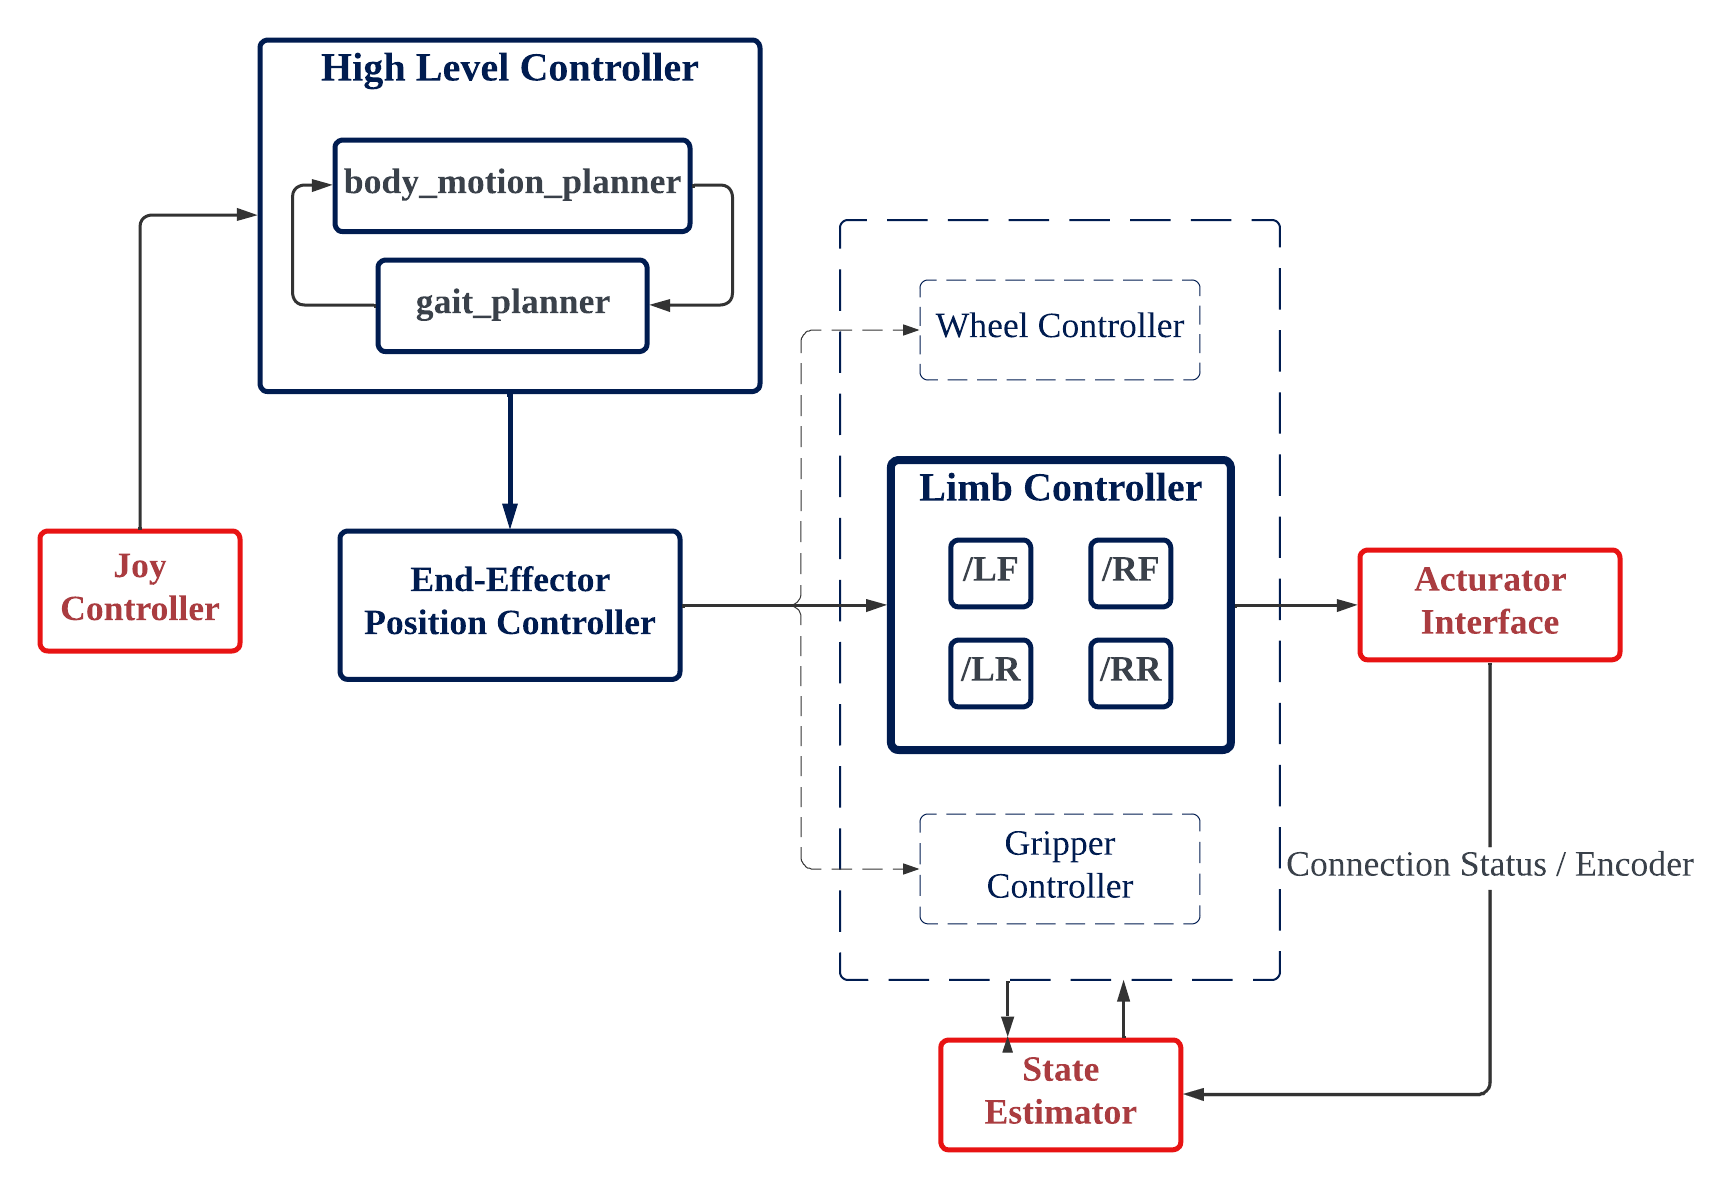
\includegraphics[width=145mm]{./fig/flowchart/Controlcolor.png}
  \vspace{2mm}
  \caption{Control architecture for full configuration Moonbot.}\label{control}
\end{figure}


\subsection{Body Movement}
The body position control is managed by the body planner, which plays a critical role in maintaining balance during locomotion and in navigating uncertain terrain. \fig{slant} shows the translational movement of the body in four directions, while \fig{rot} depicts its rotation around three axes. \\

\begin{figure}[ht]
    \centering
    \begin{subfigure}[b]{0.45\textwidth}
        \centering
        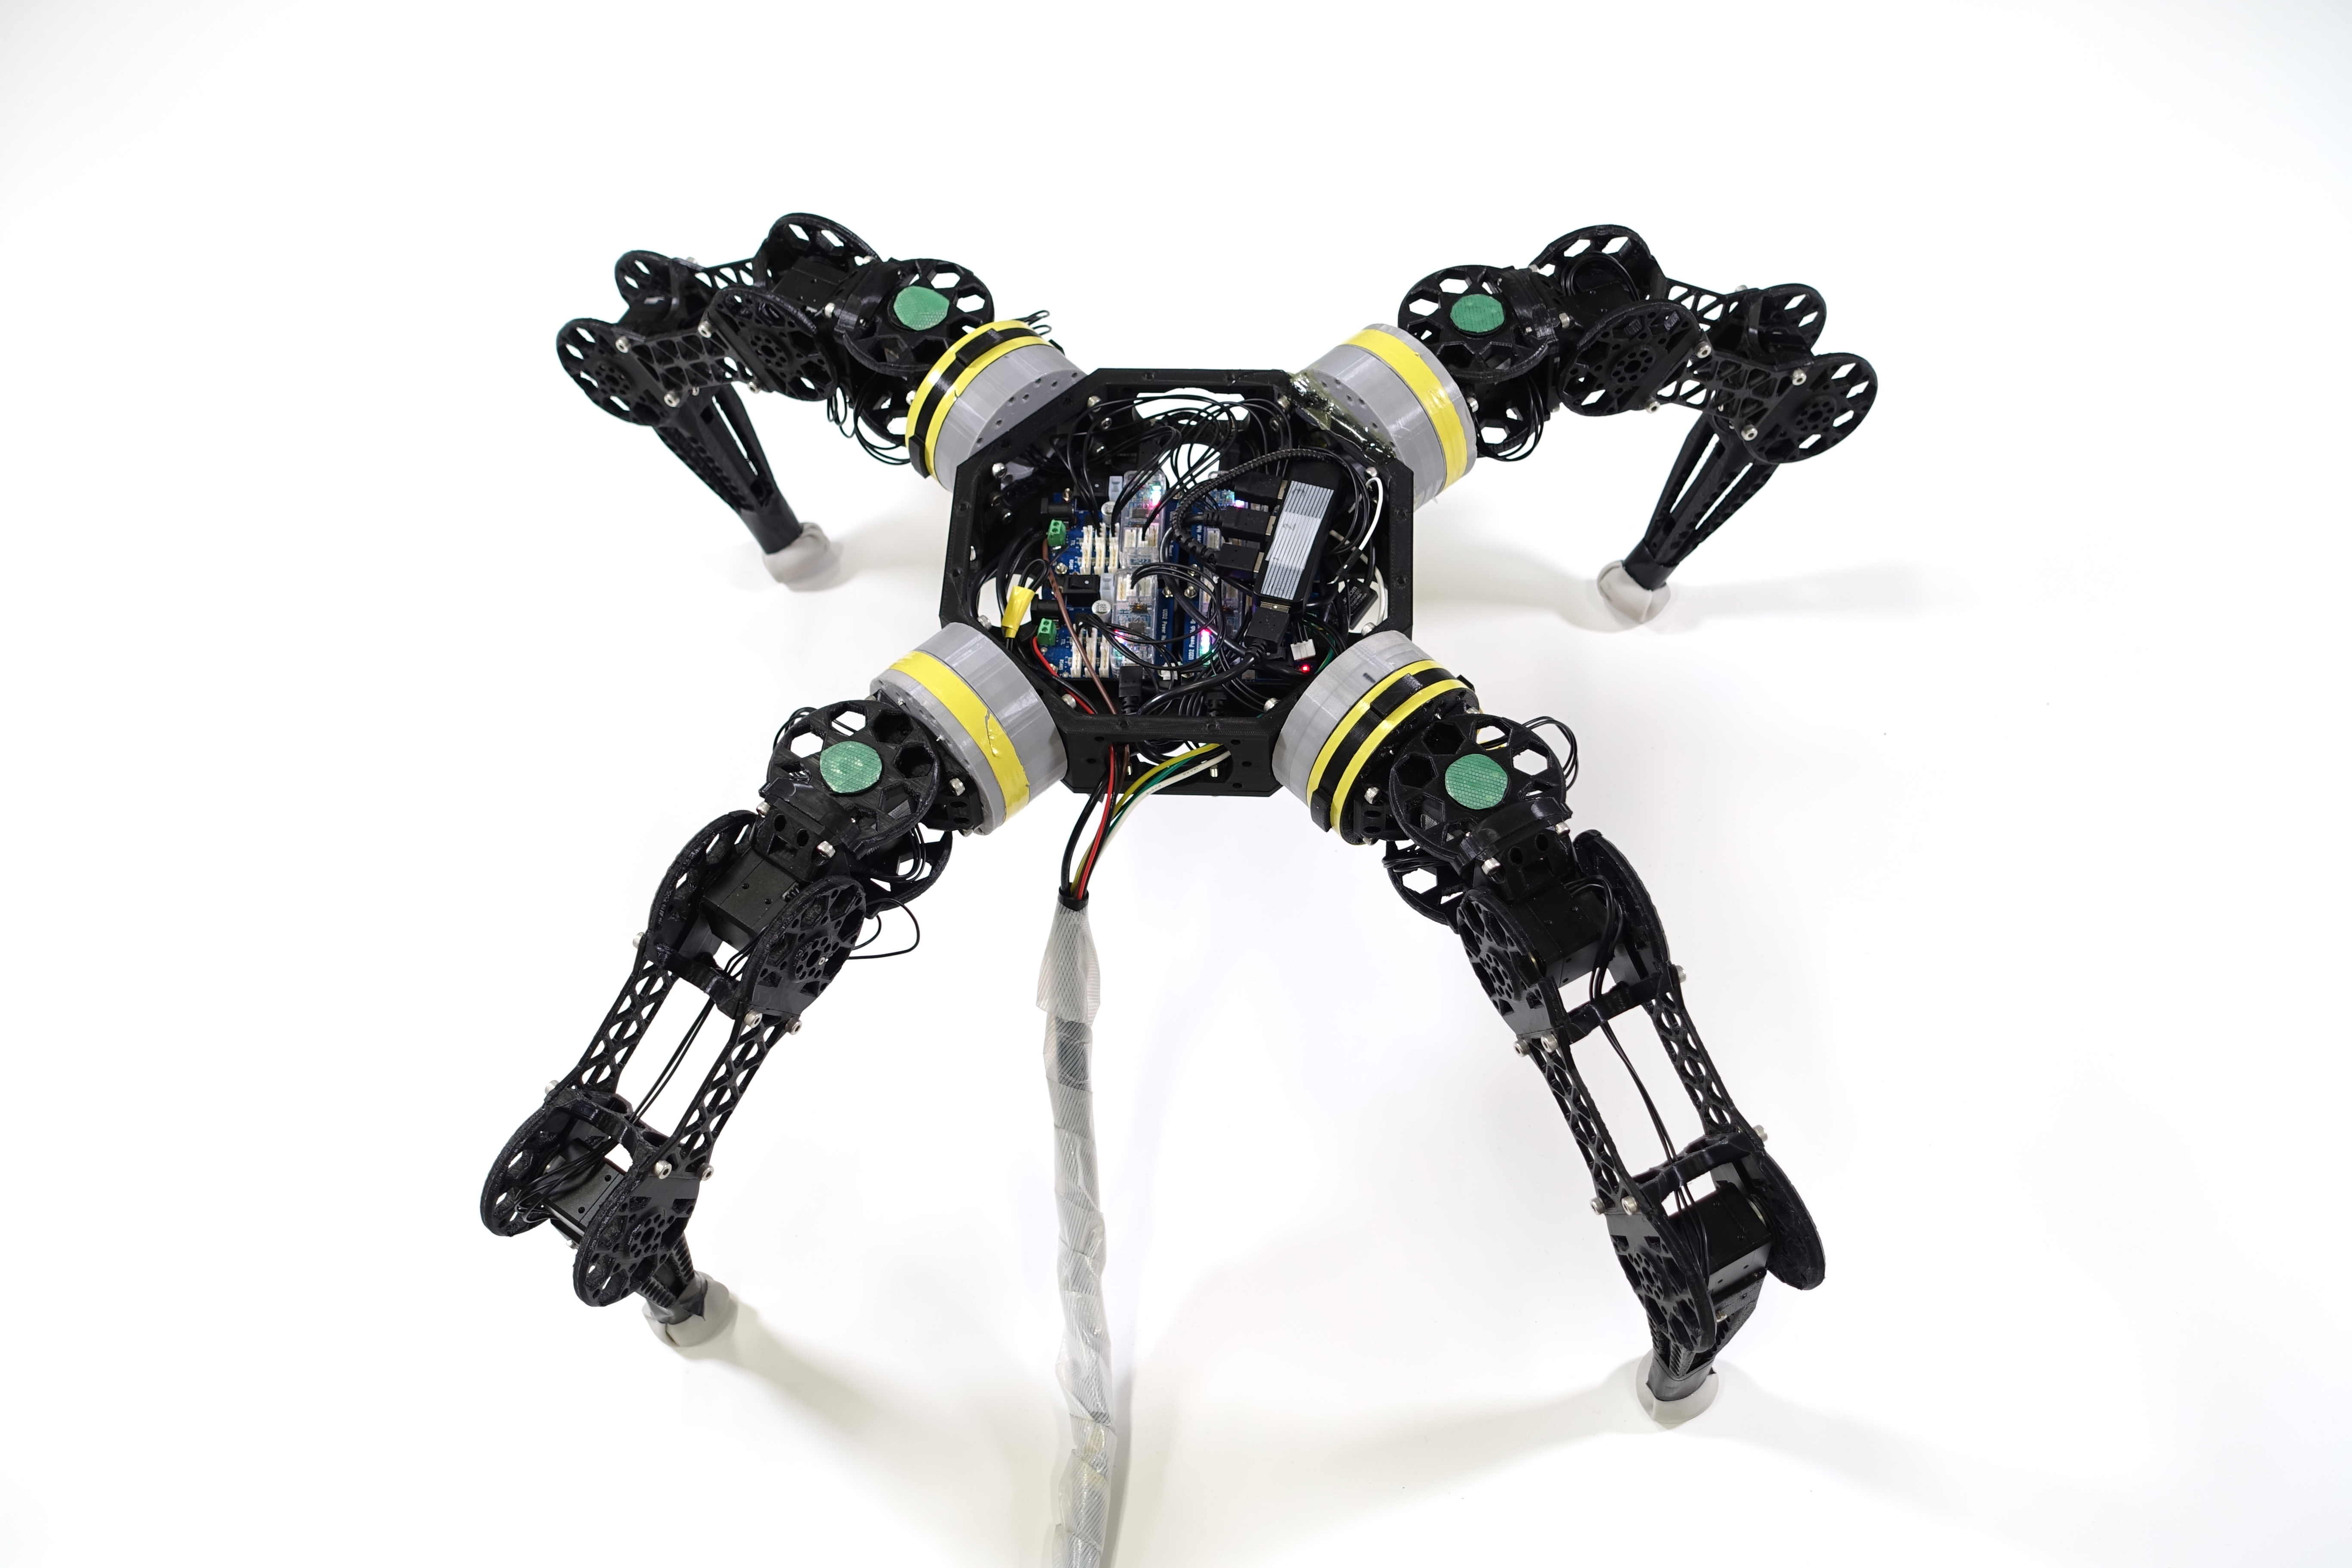
\includegraphics[width=70mm]{./fig/chap4/body_movement/front05cmslant.JPG}
        \caption{Body moves 5 cm to the front.}
        \label{slantfront}
    \end{subfigure}
    \begin{subfigure}[b]{0.45\textwidth}
        \centering
        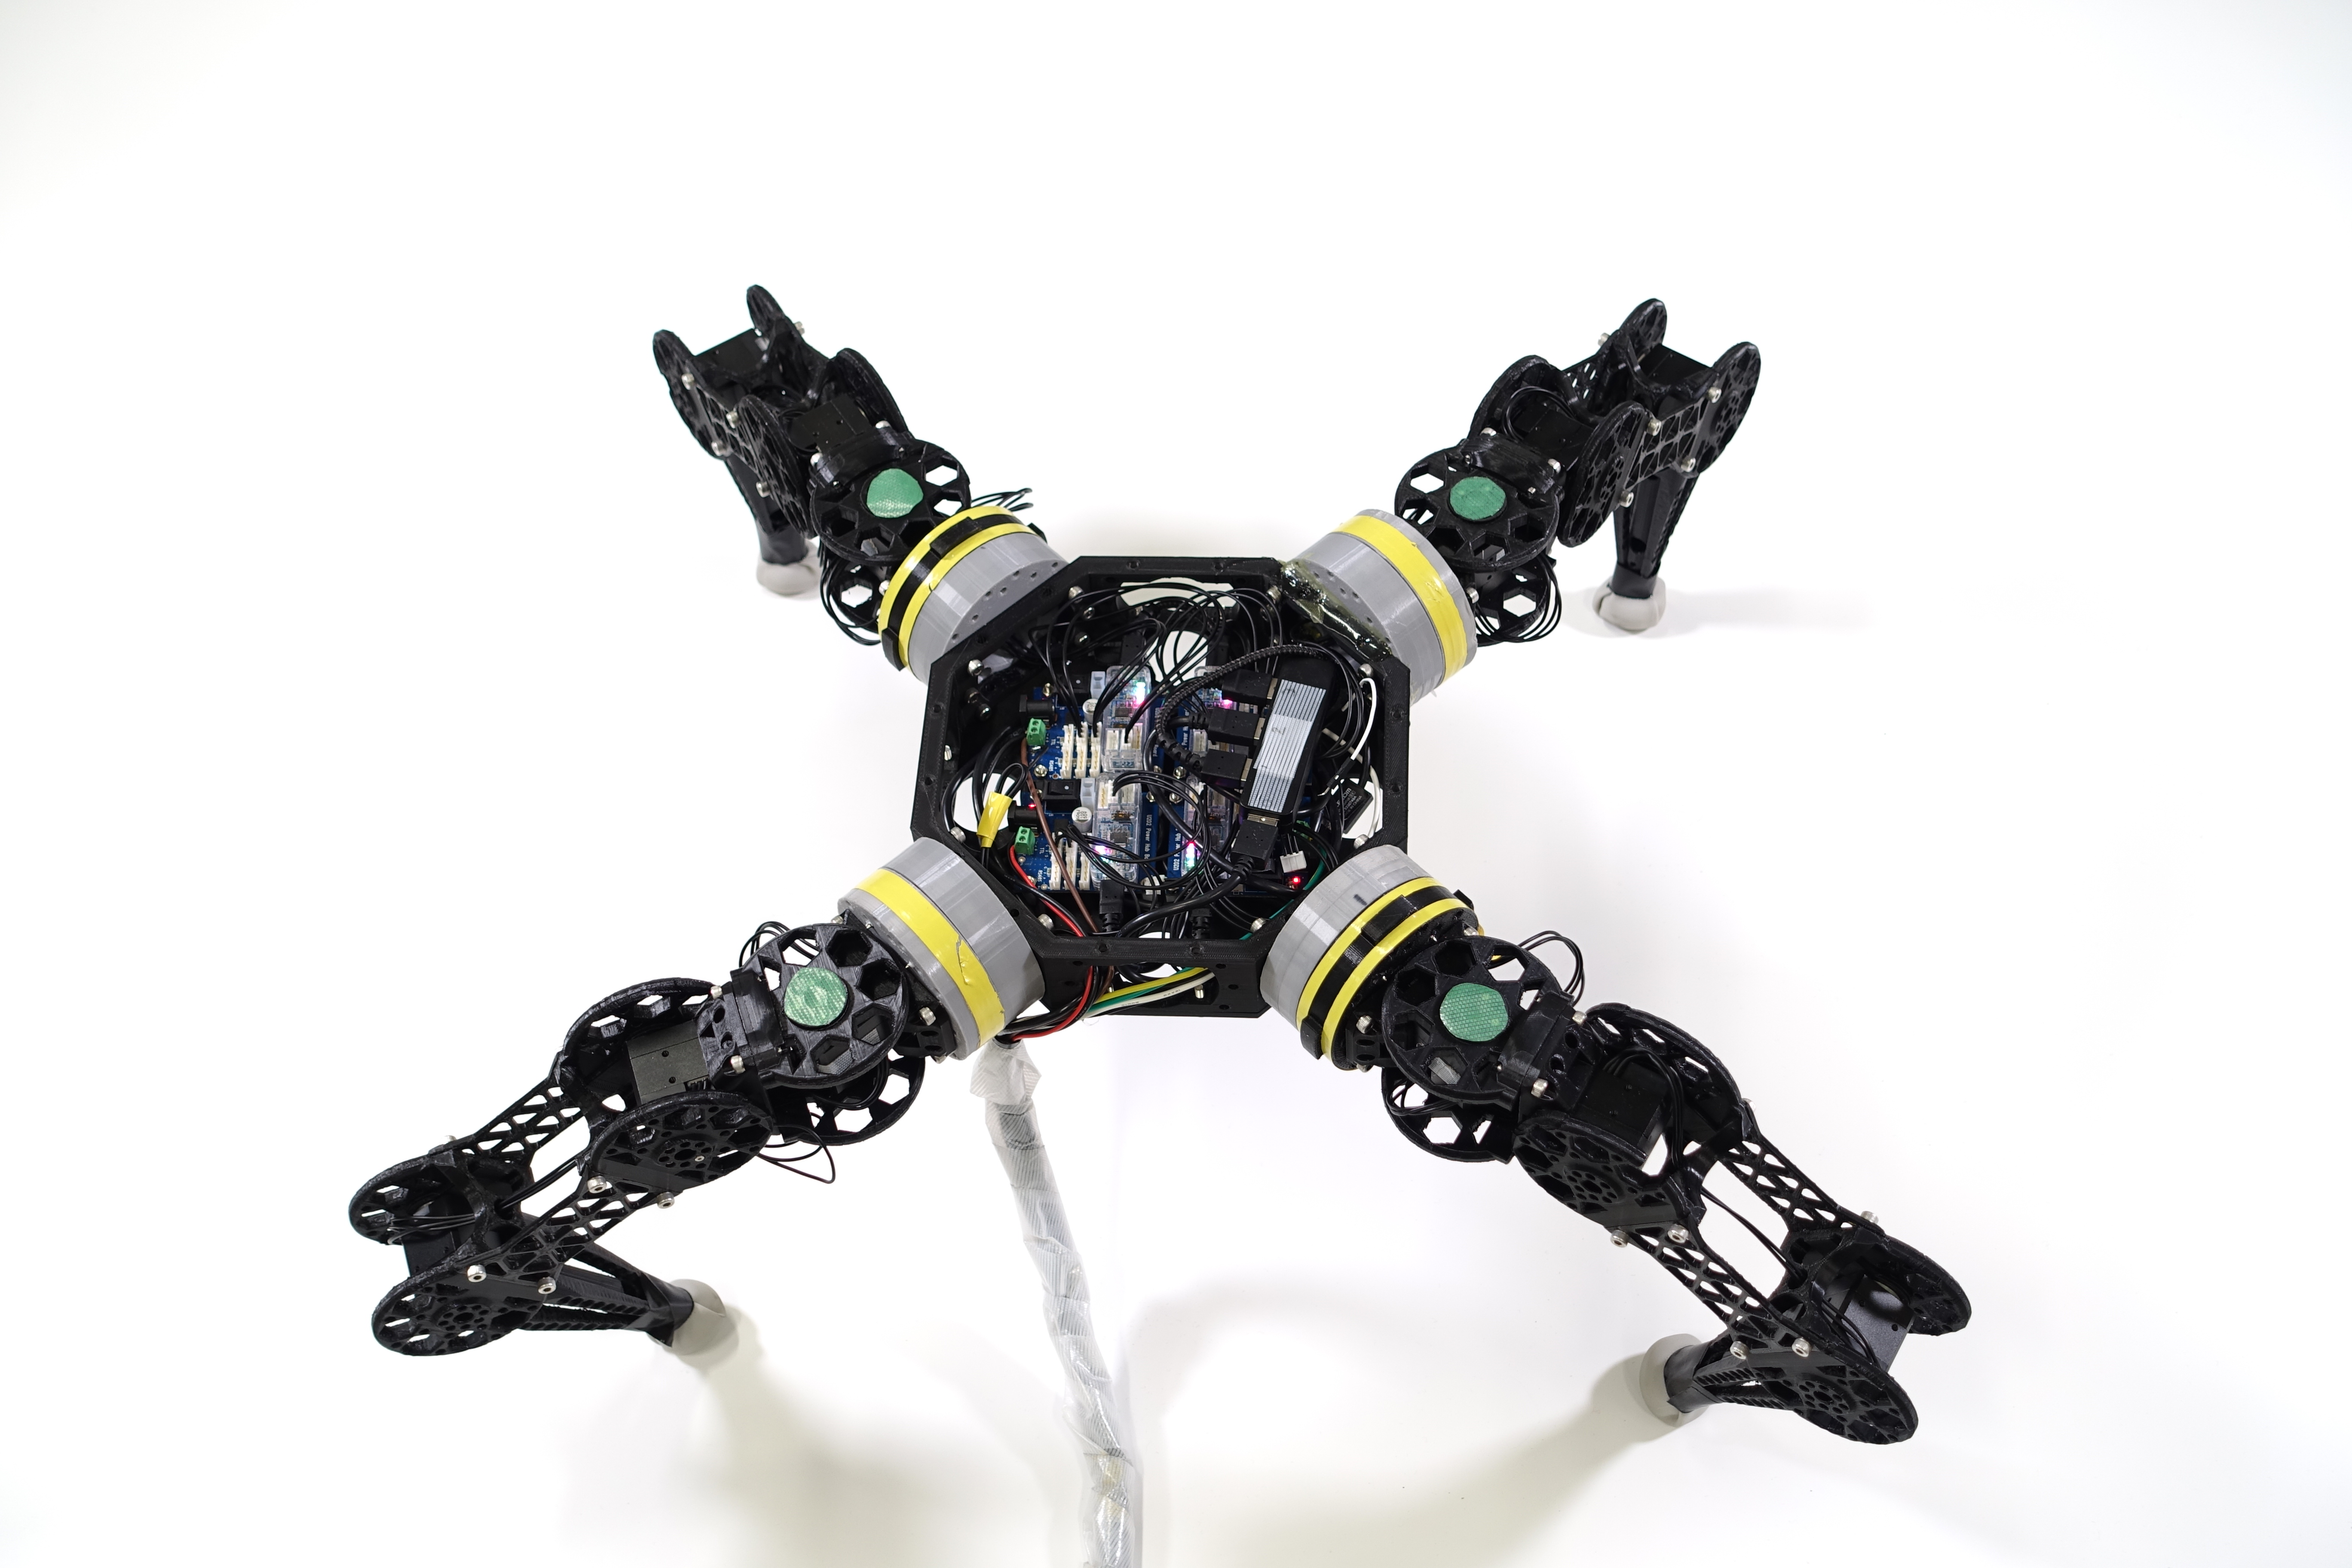
\includegraphics[width=70mm]{./fig/chap4/body_movement/back05cmslant.JPG}
        \caption{Body moves 5 cm to the back.}
        \label{slantback}
    \end{subfigure}
    \\
    \begin{subfigure}[b]{0.45\textwidth}
        \centering
        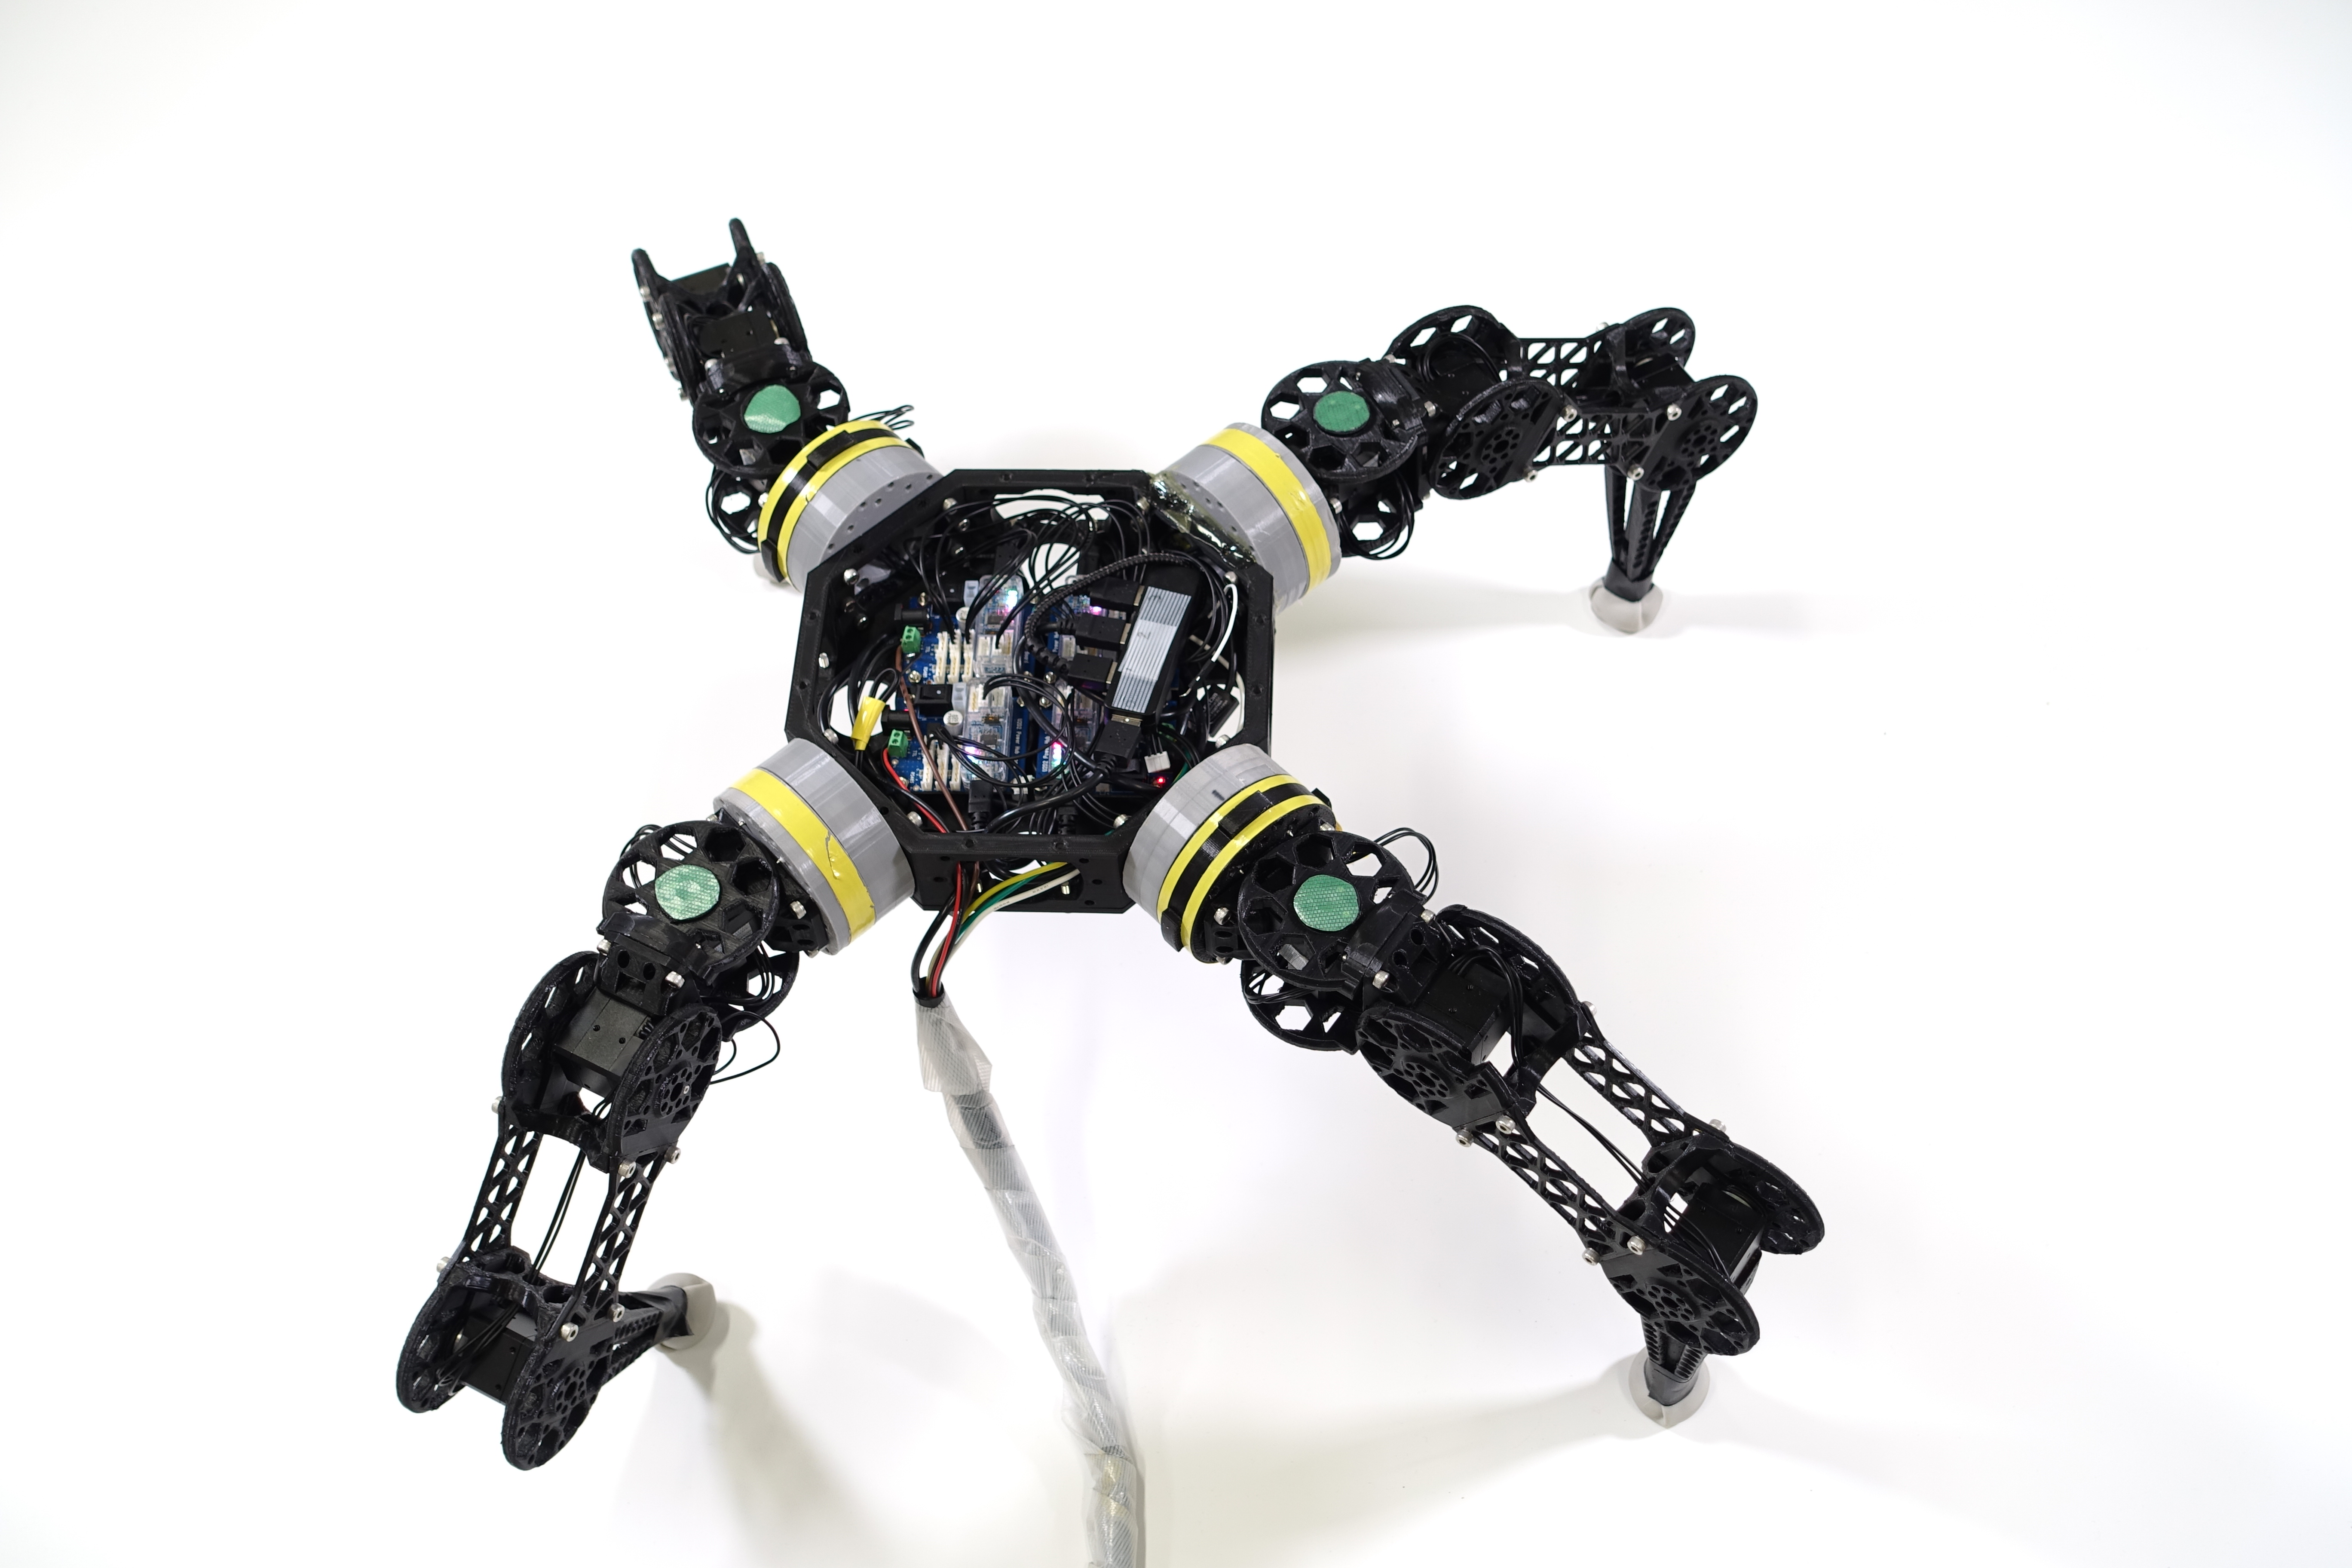
\includegraphics[width=70mm]{./fig/chap4/body_movement/left05cmslant.JPG}
        \caption{Body moves 5 cm to the left.}
        \label{slantleft}
    \end{subfigure}
    \begin{subfigure}[b]{0.45\textwidth}
        \centering
        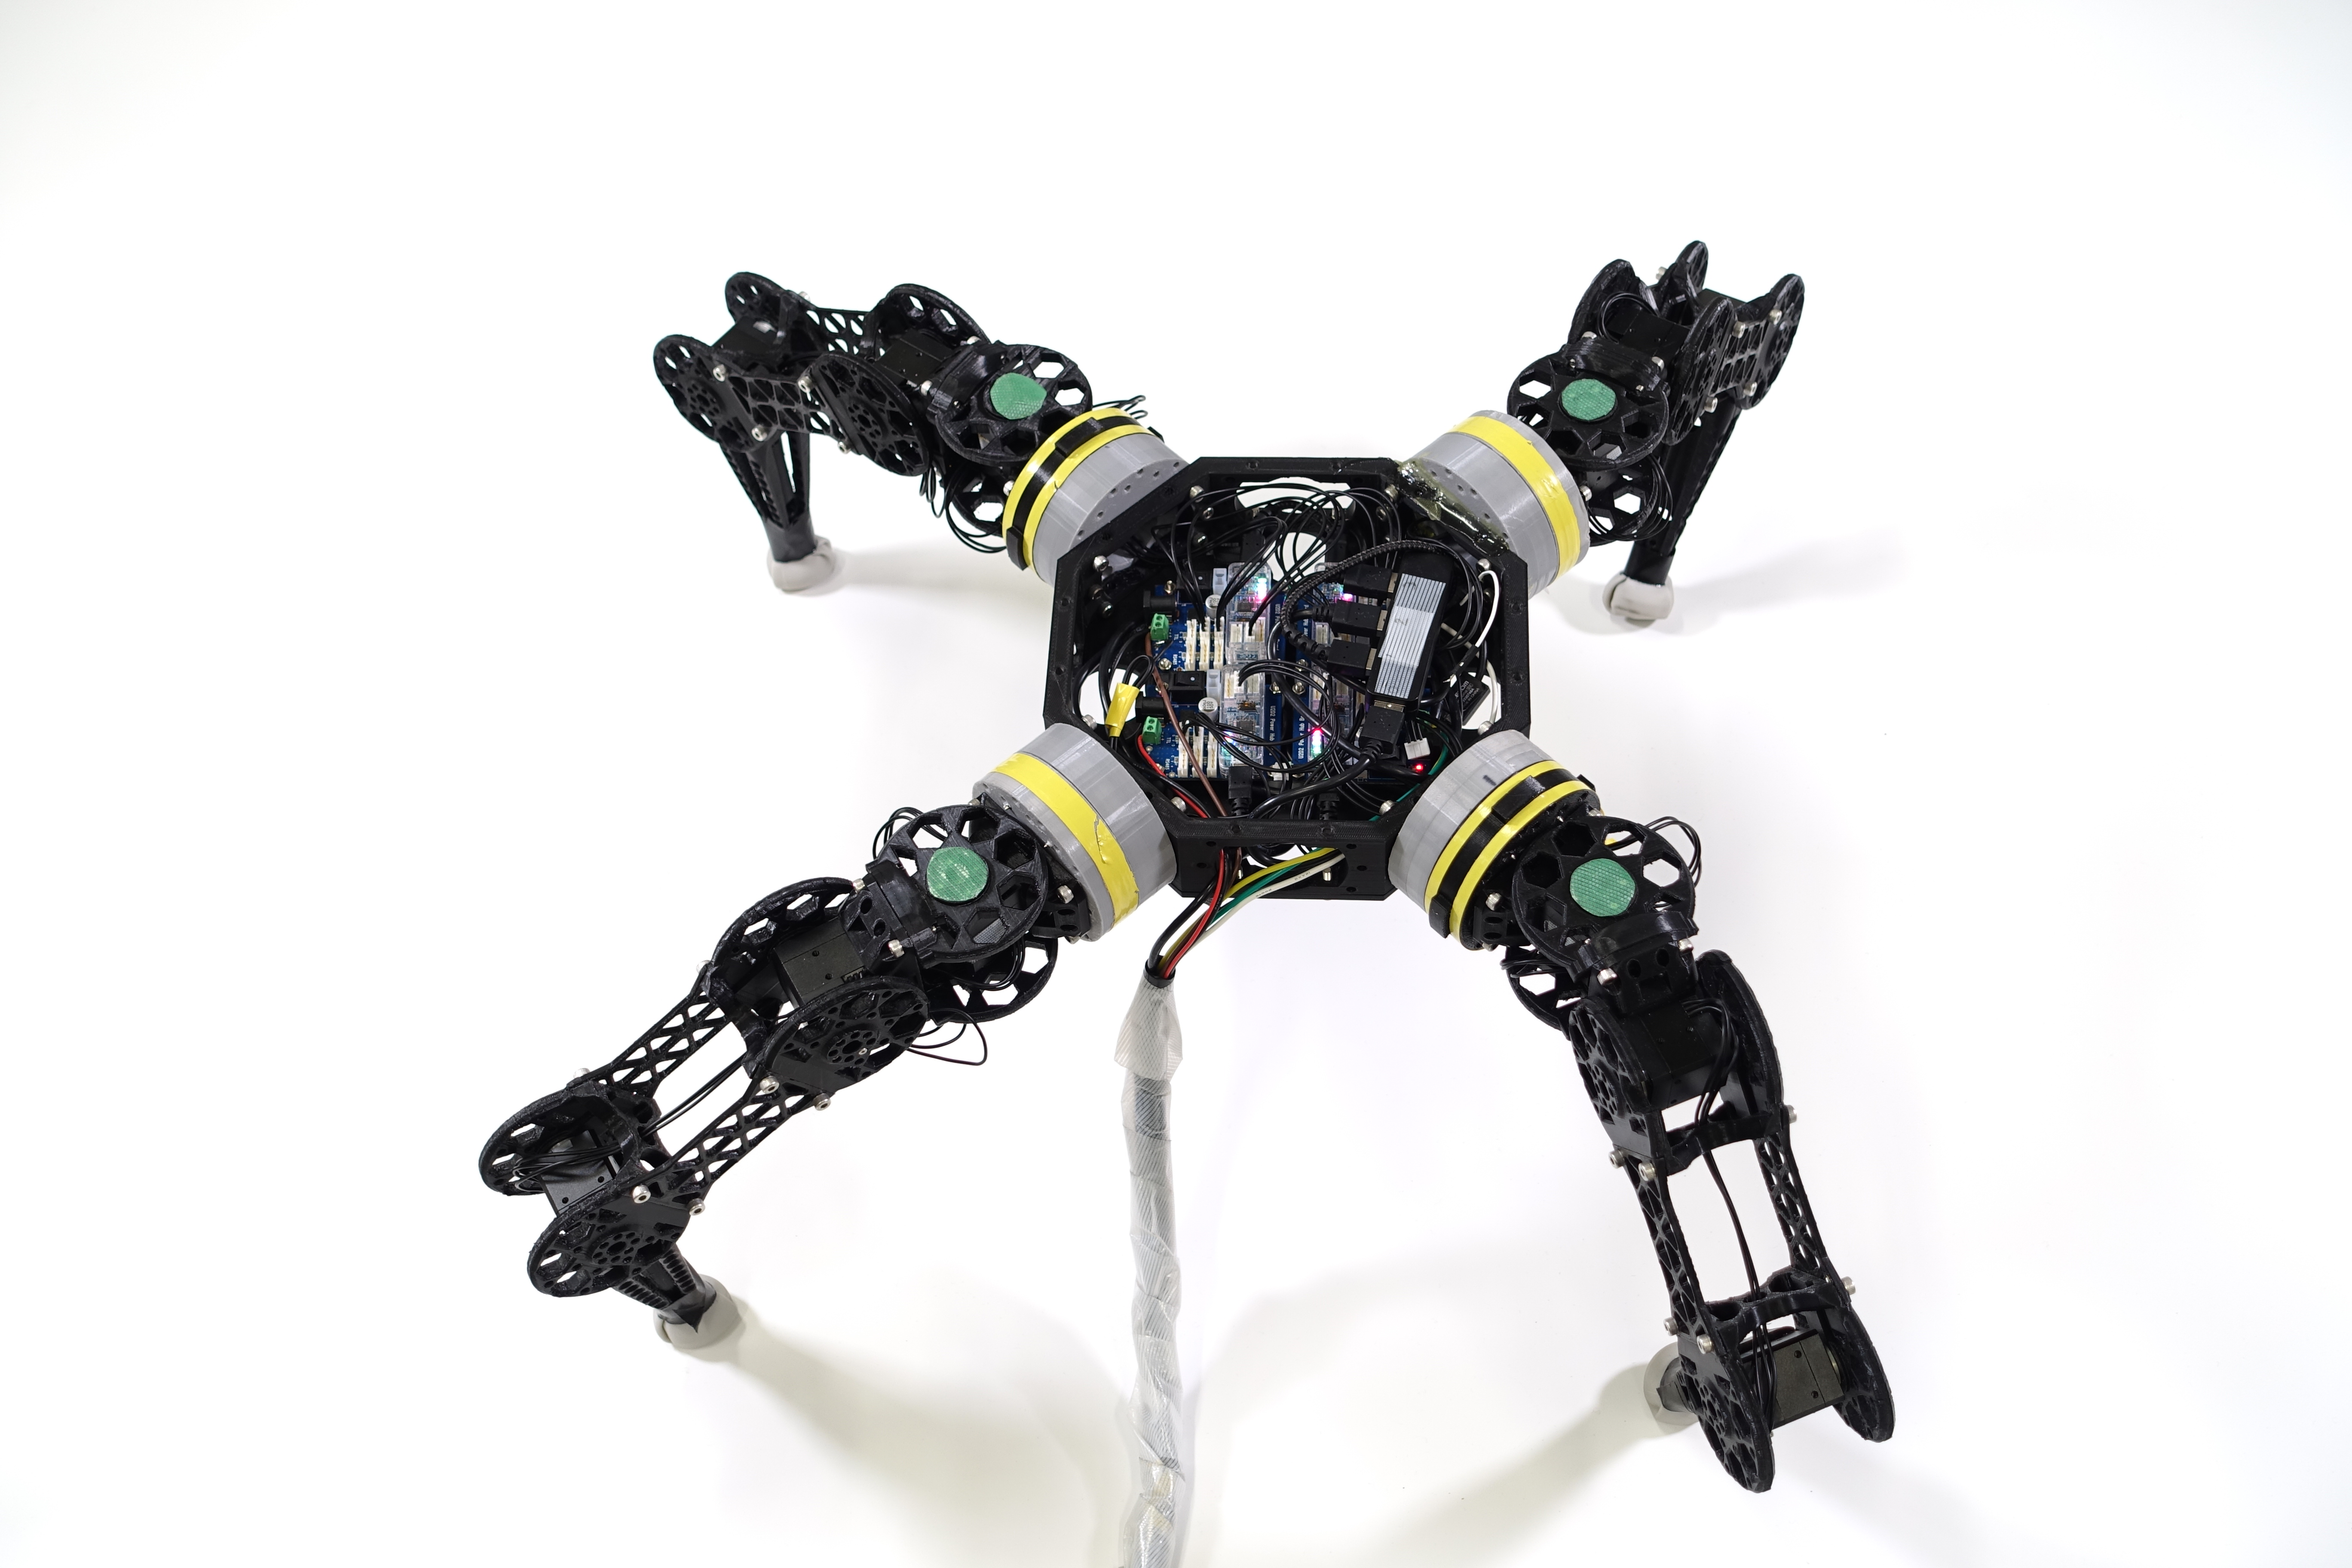
\includegraphics[width=70mm]{./fig/chap4/body_movement/right05cmslant.JPG}
        \caption{Body moves 5 cm to the right.}
        \label{slantright}
    \end{subfigure}
    \caption{Body translational movement.}
    \label{slant}
\end{figure}

\begin{figure}[ht]
    \centering
    \begin{subfigure}[b]{0.45\textwidth}
        \centering
        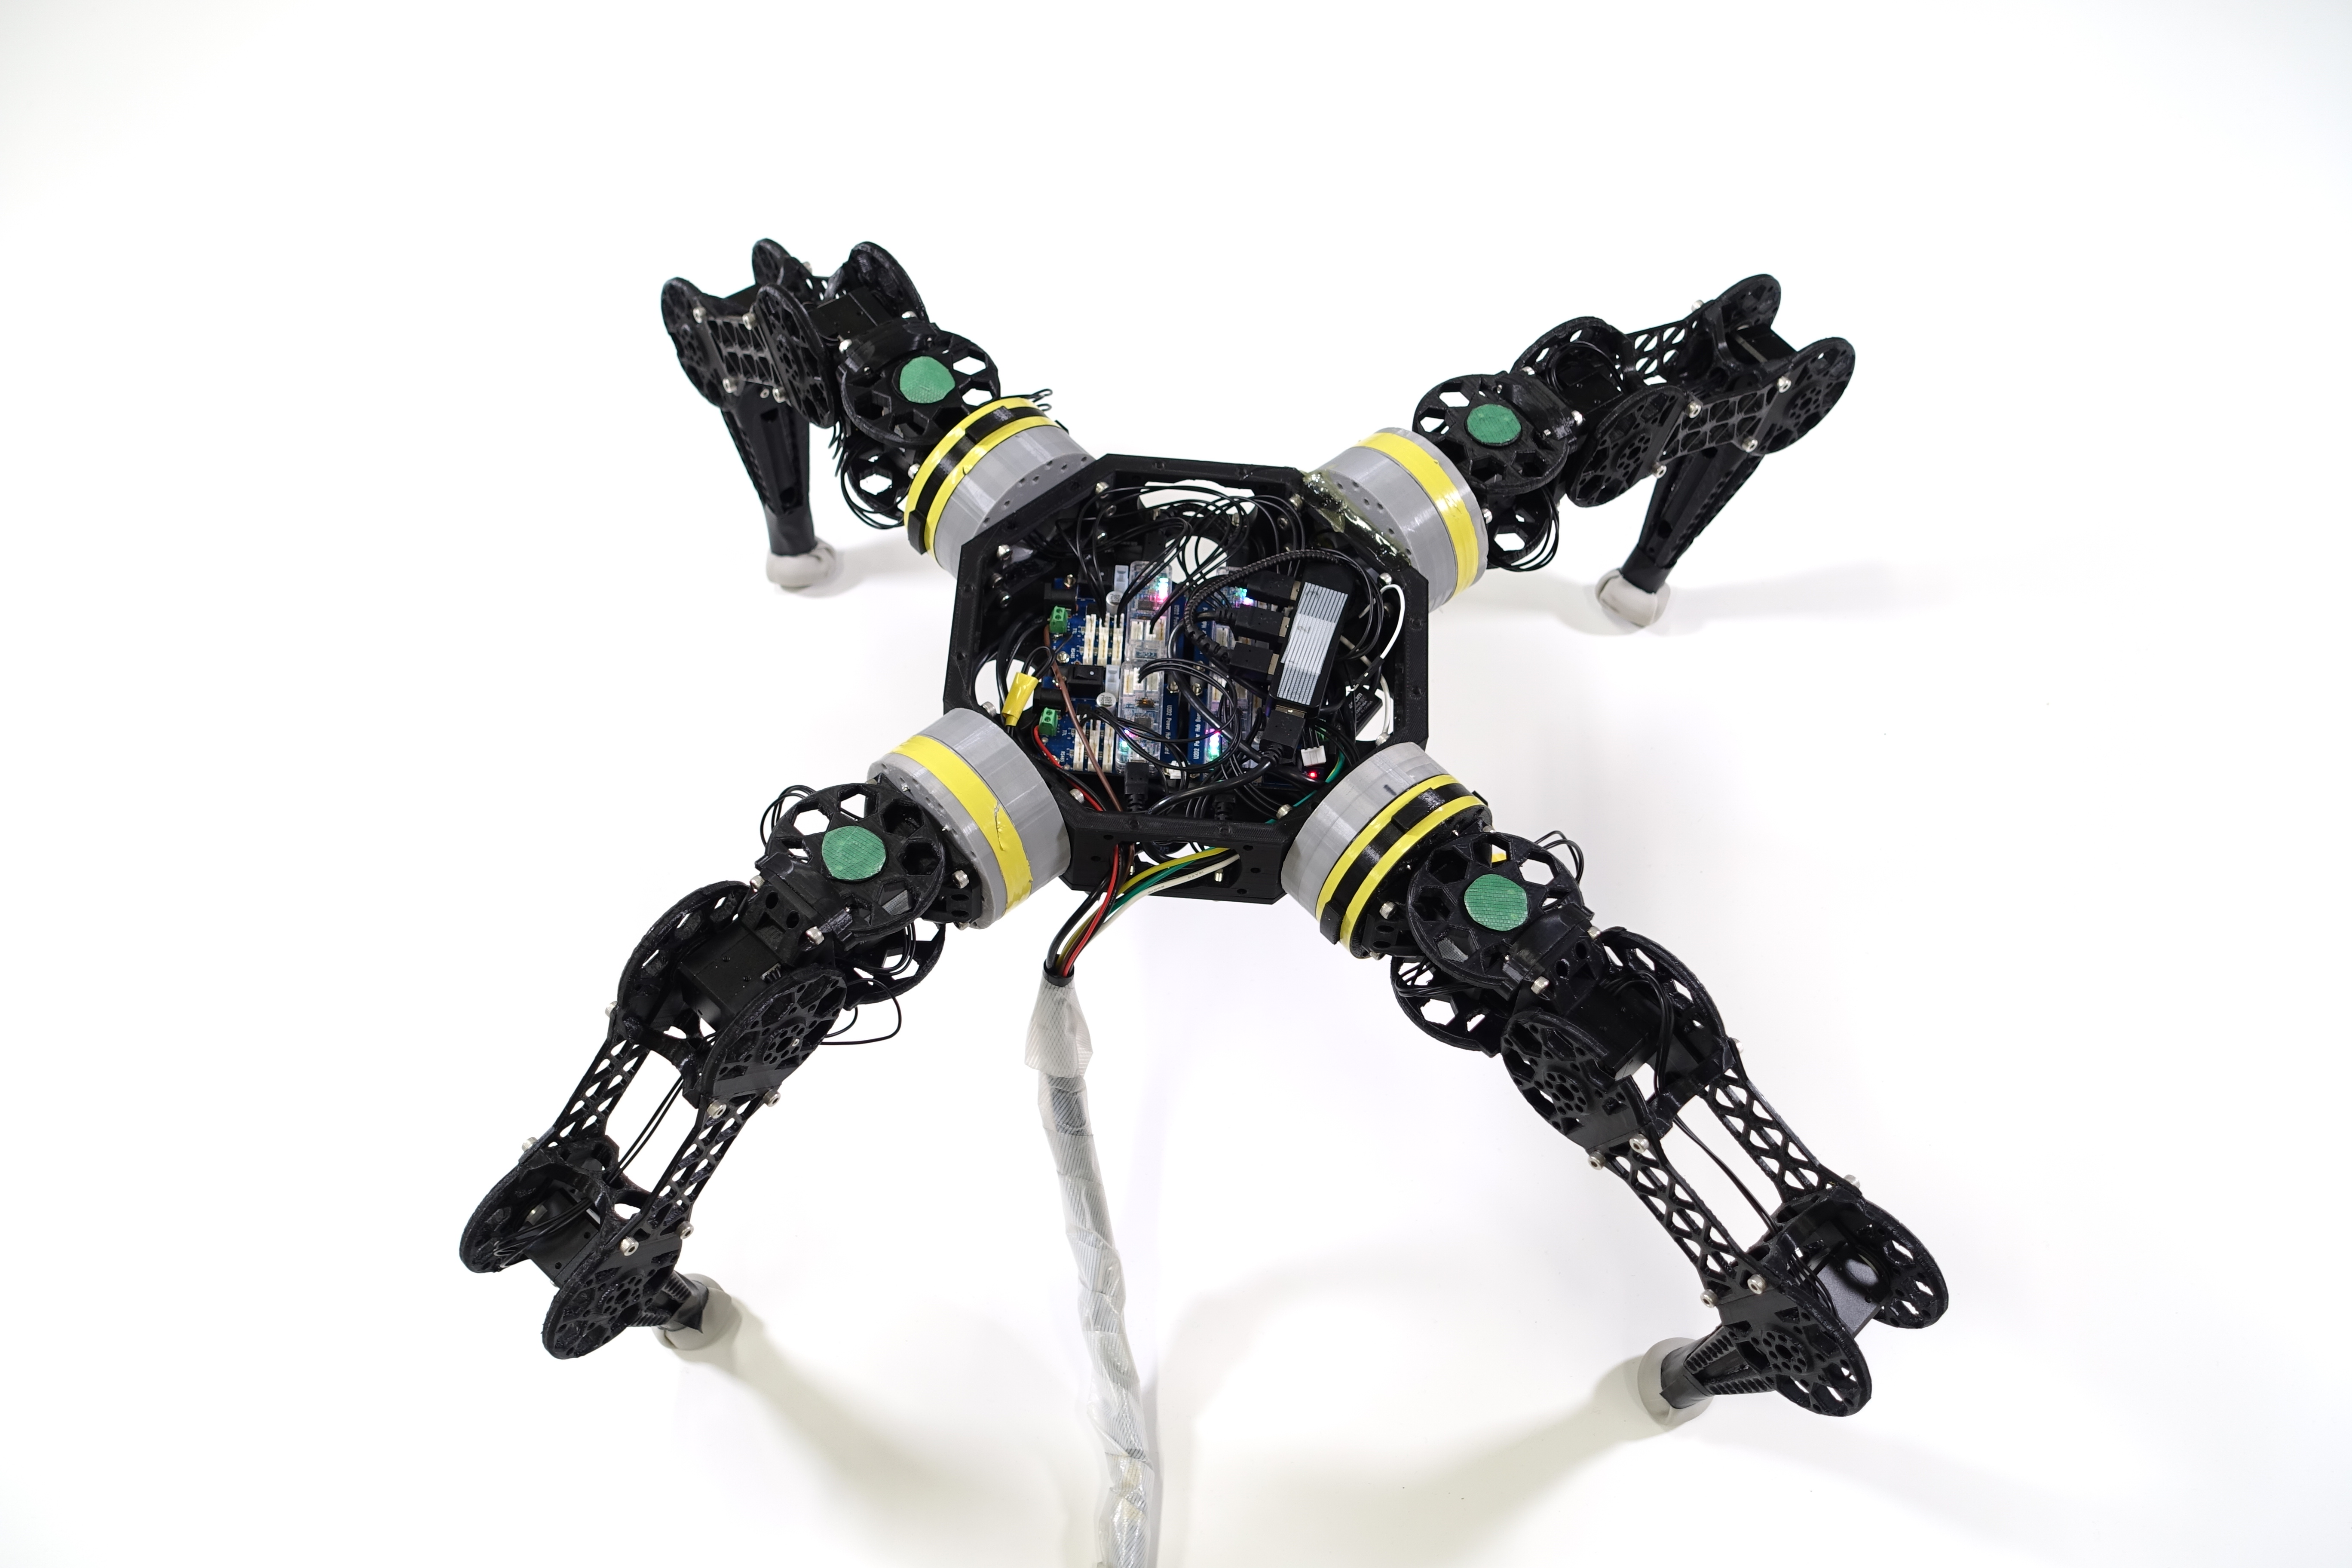
\includegraphics[width=70mm]{./fig/chap4/body_movement/p05roll.JPG}
        \caption{Body rotates 5 degrees in roll.}
        \label{protroll}
    \end{subfigure}
    \begin{subfigure}[b]{0.45\textwidth}
        \centering
        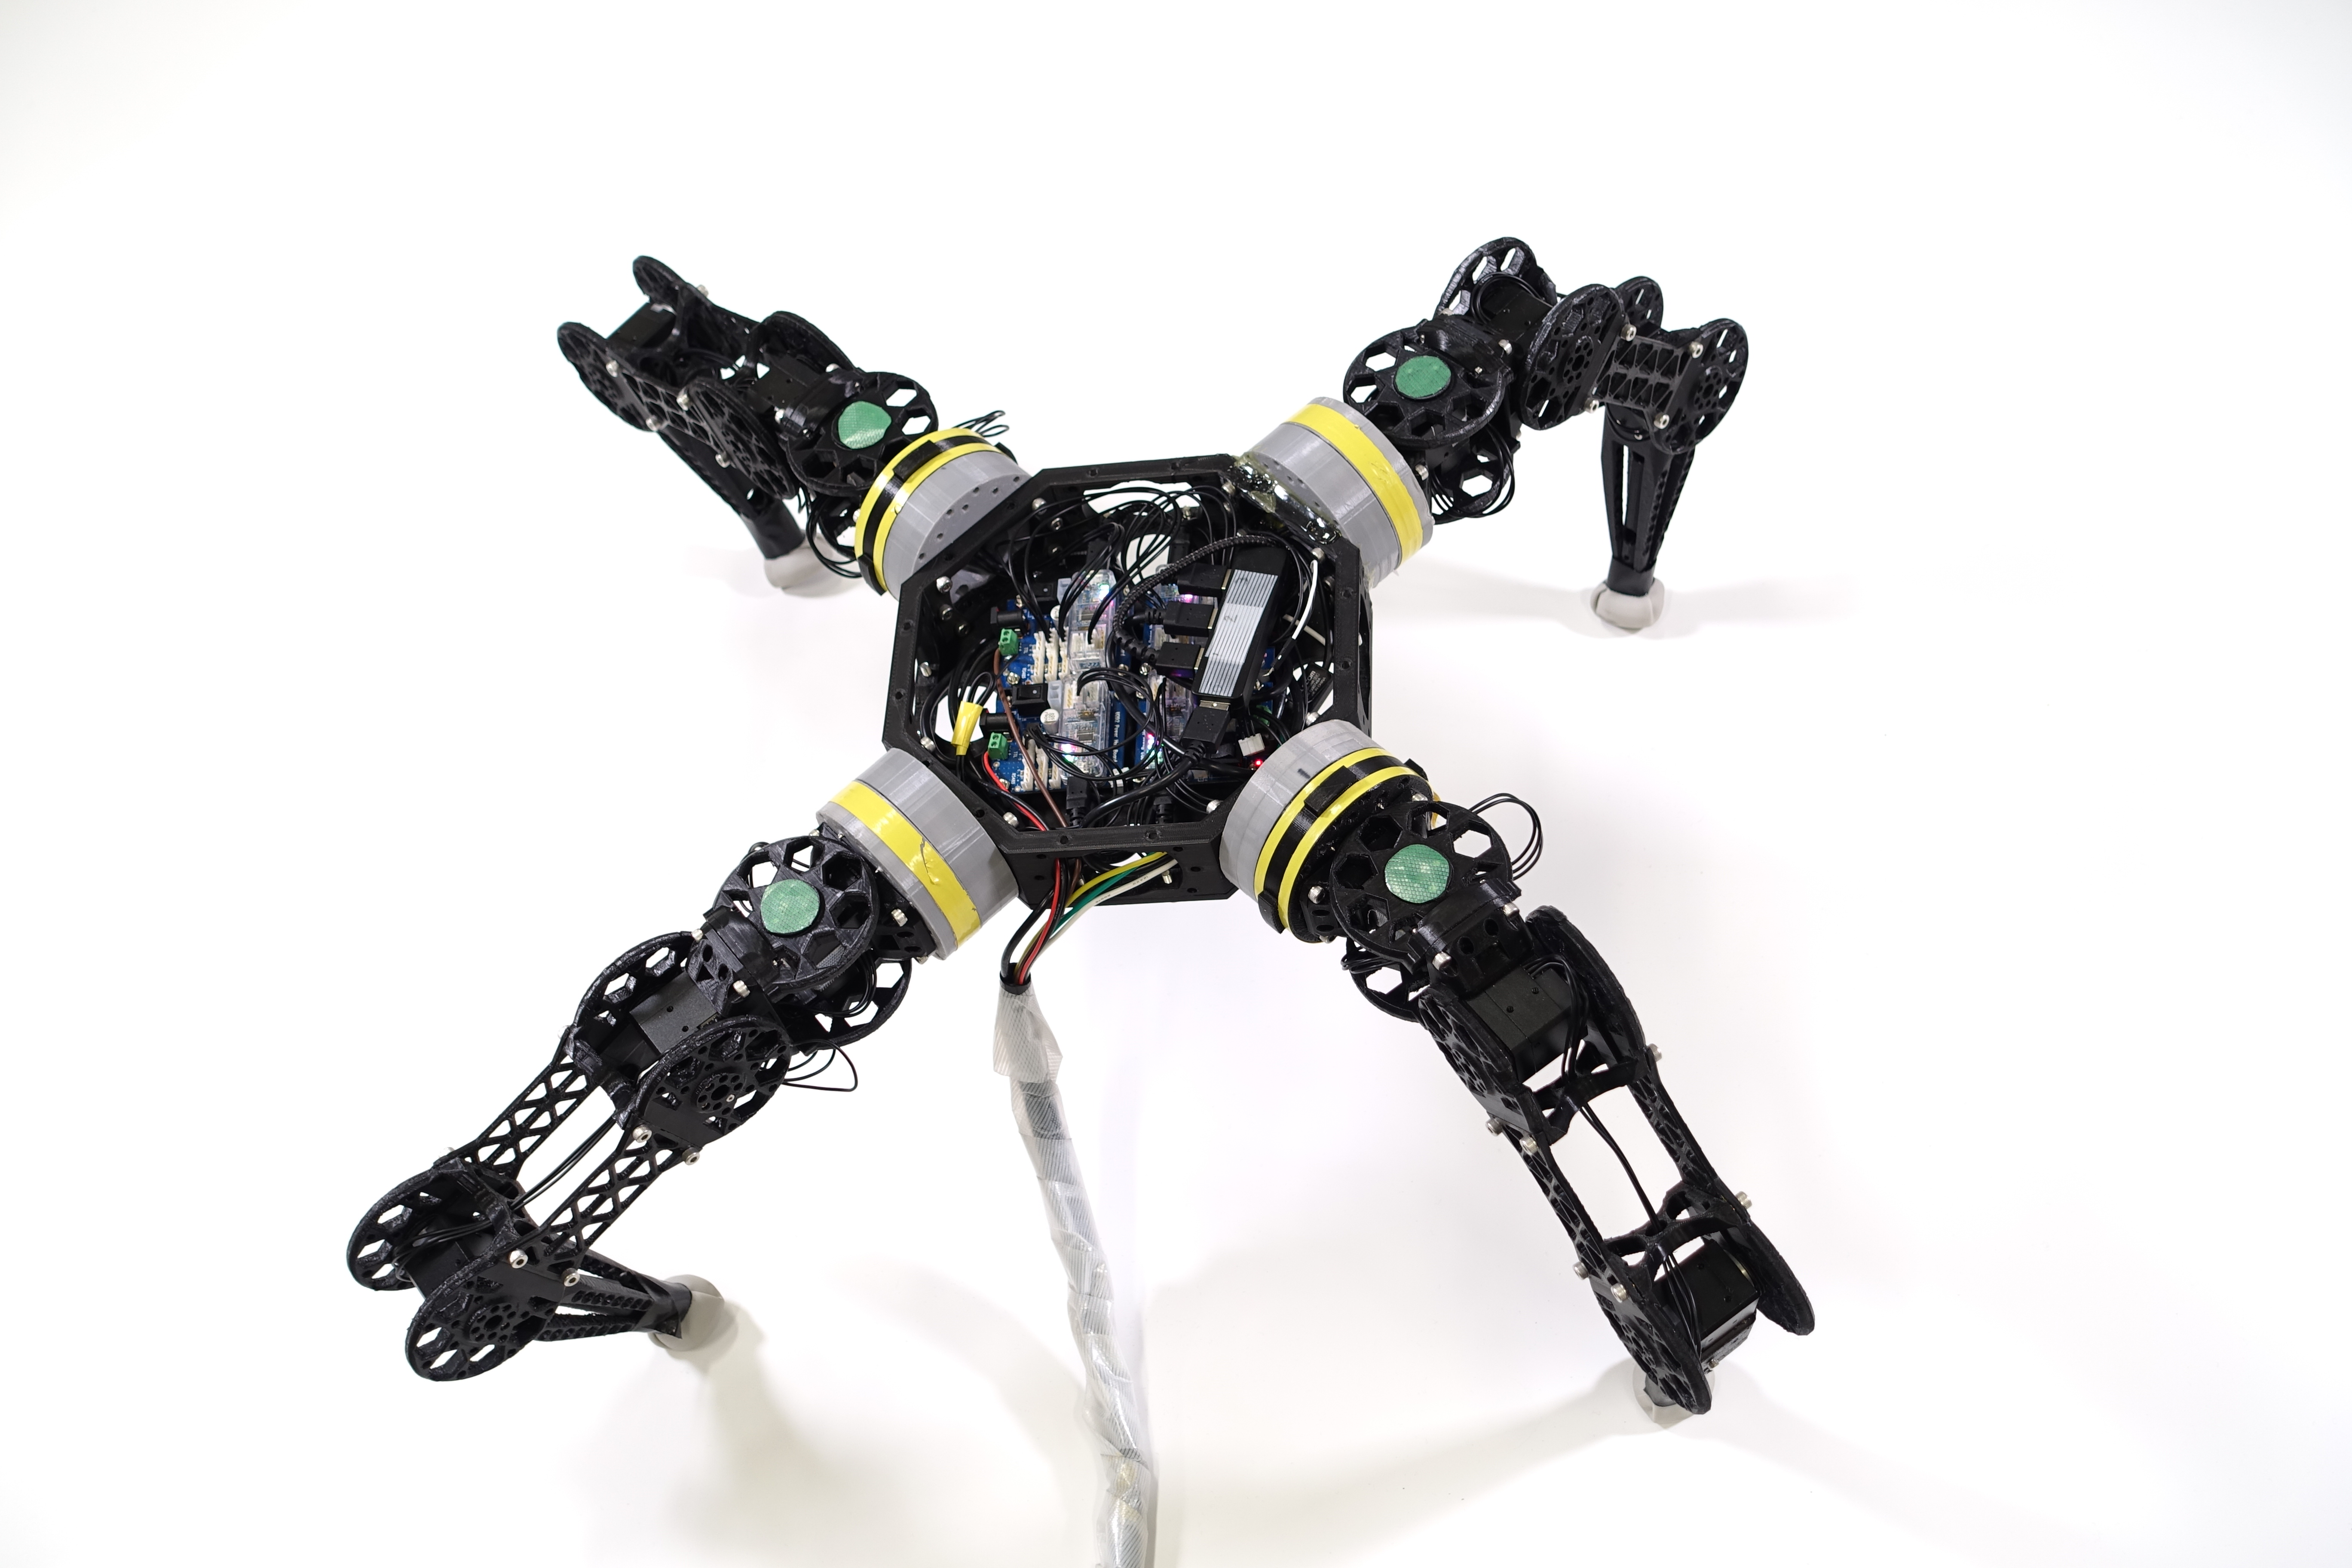
\includegraphics[width=70mm]{./fig/chap4/body_movement/n05roll.JPG}
        \caption{Body rotates -5 degrees in roll.}
        \label{nrotroll}
    \end{subfigure}
    \\
    \begin{subfigure}[b]{0.45\textwidth}
        \centering
        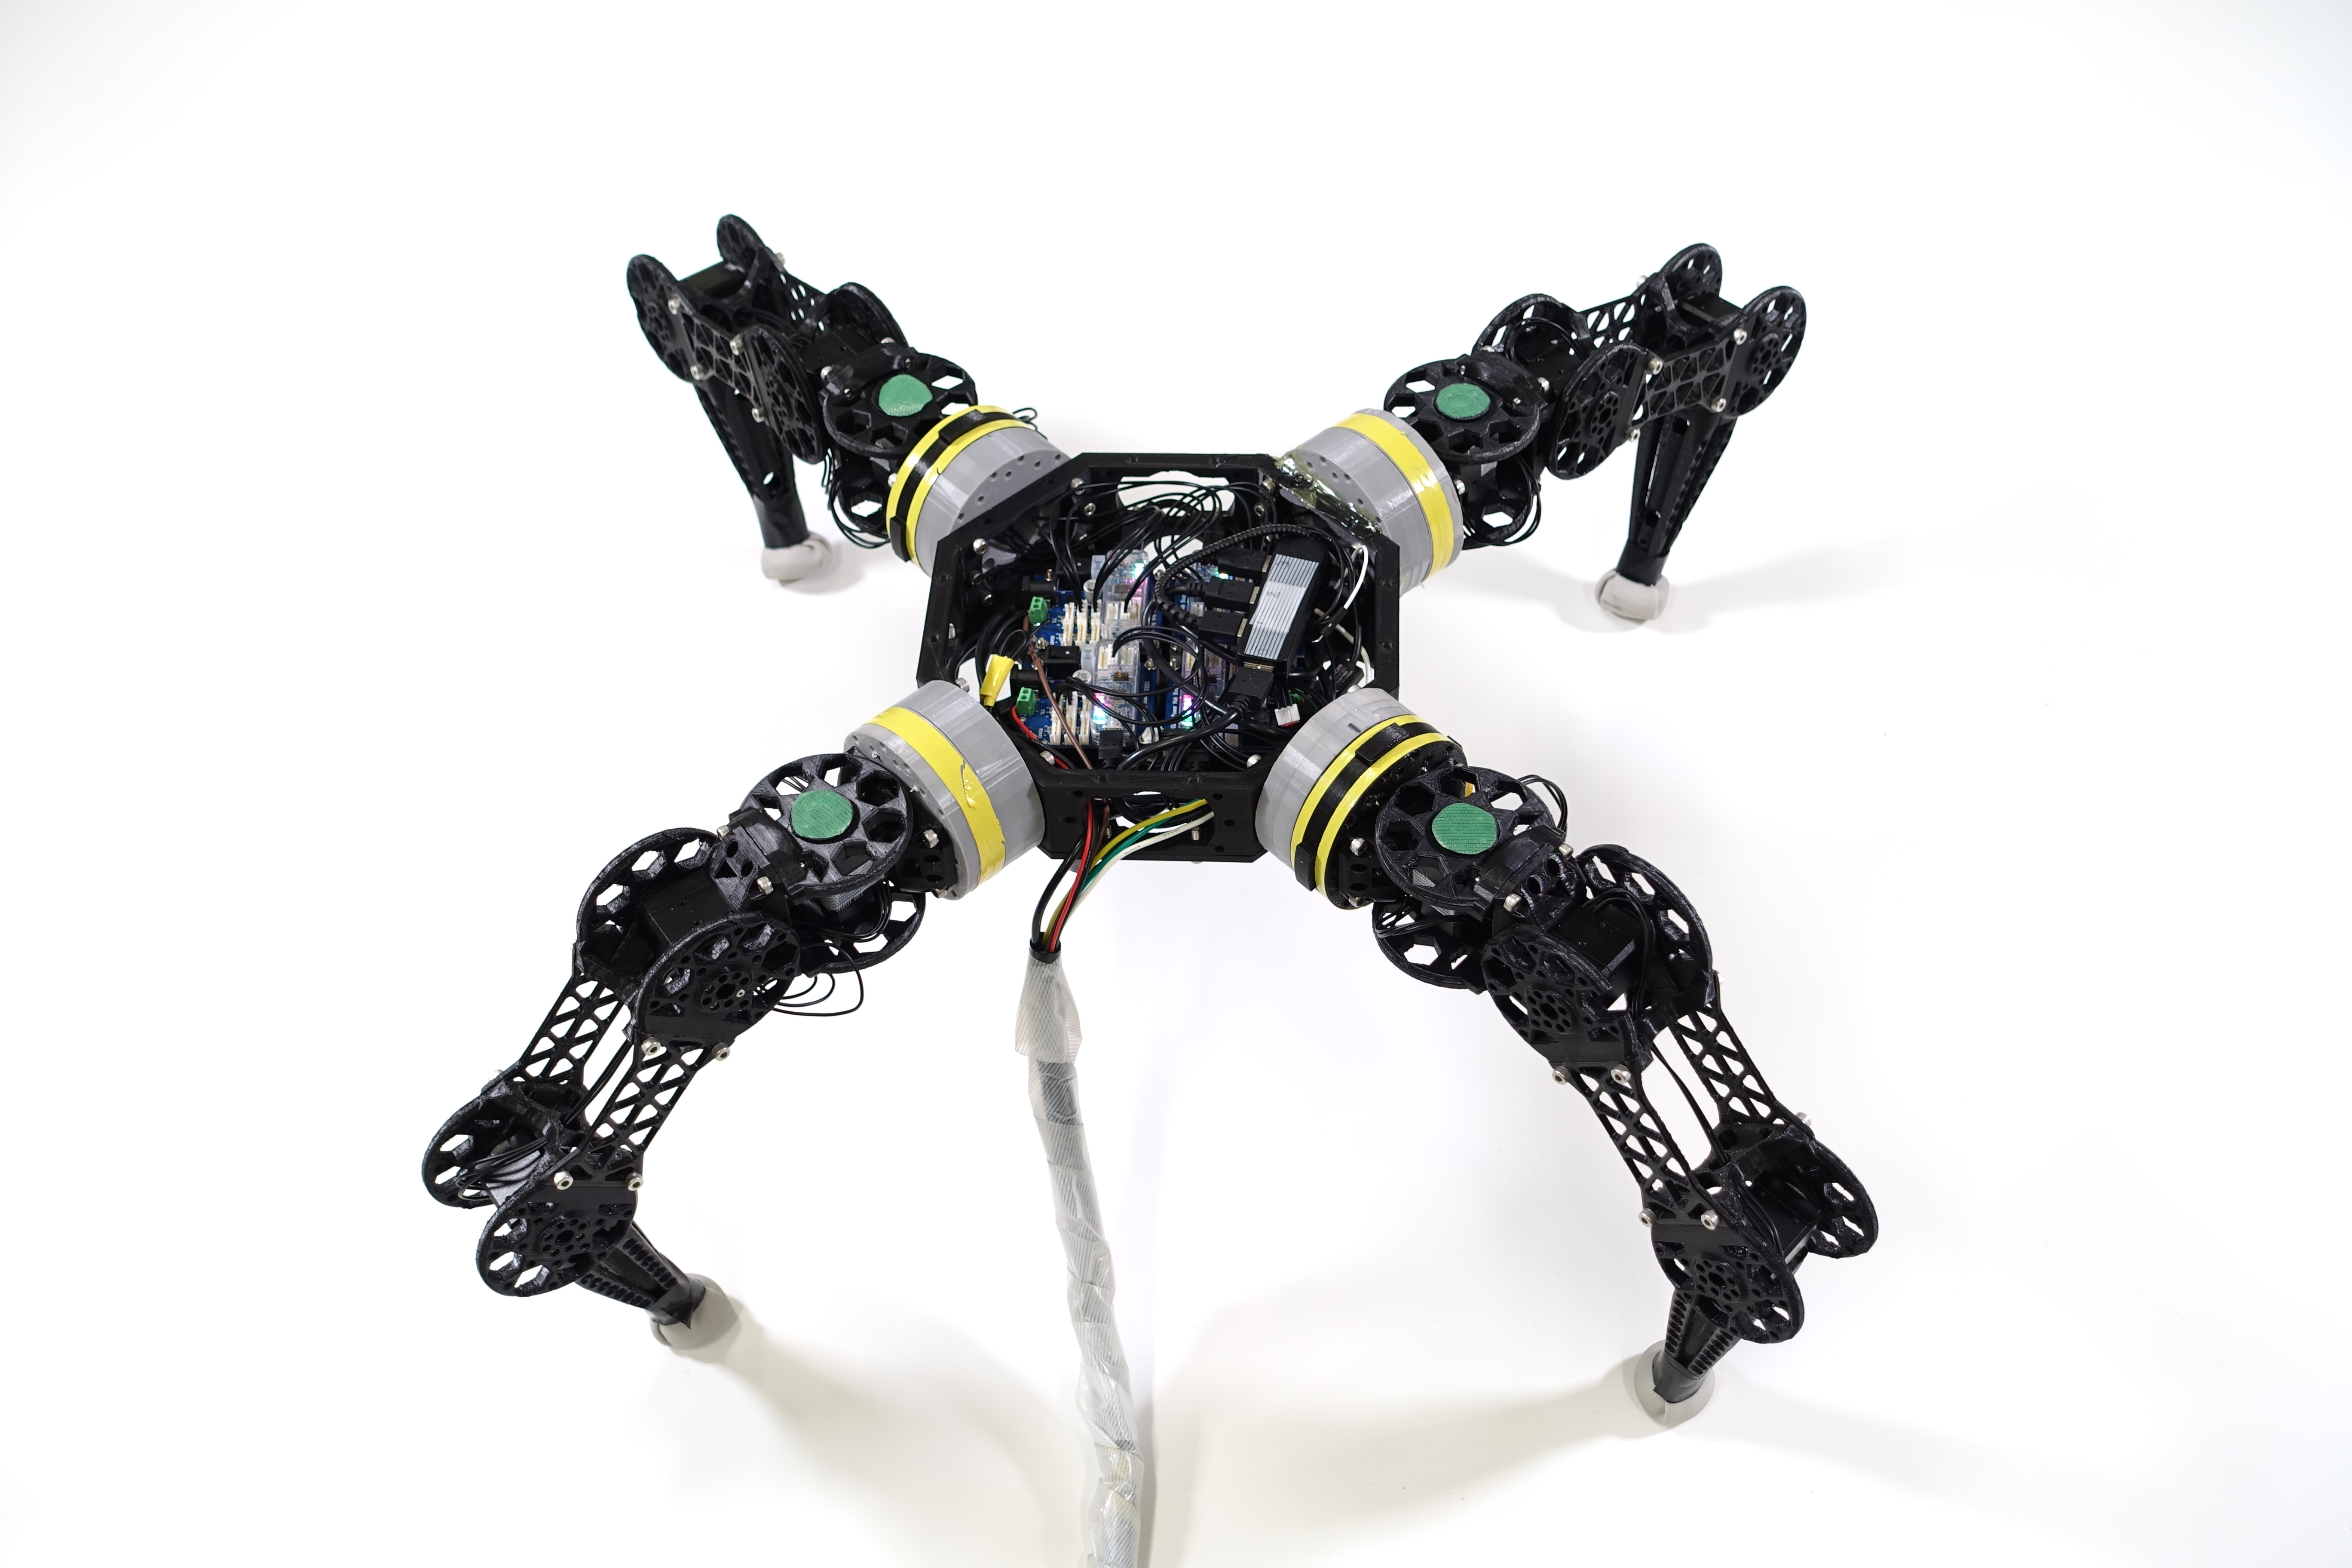
\includegraphics[width=70mm]{./fig/chap4/body_movement/p05pitch.JPG}
        \caption{Body rotates 5 degrees in pitch.}
        \label{protpitch}
    \end{subfigure}
    \begin{subfigure}[b]{0.45\textwidth}
        \centering
        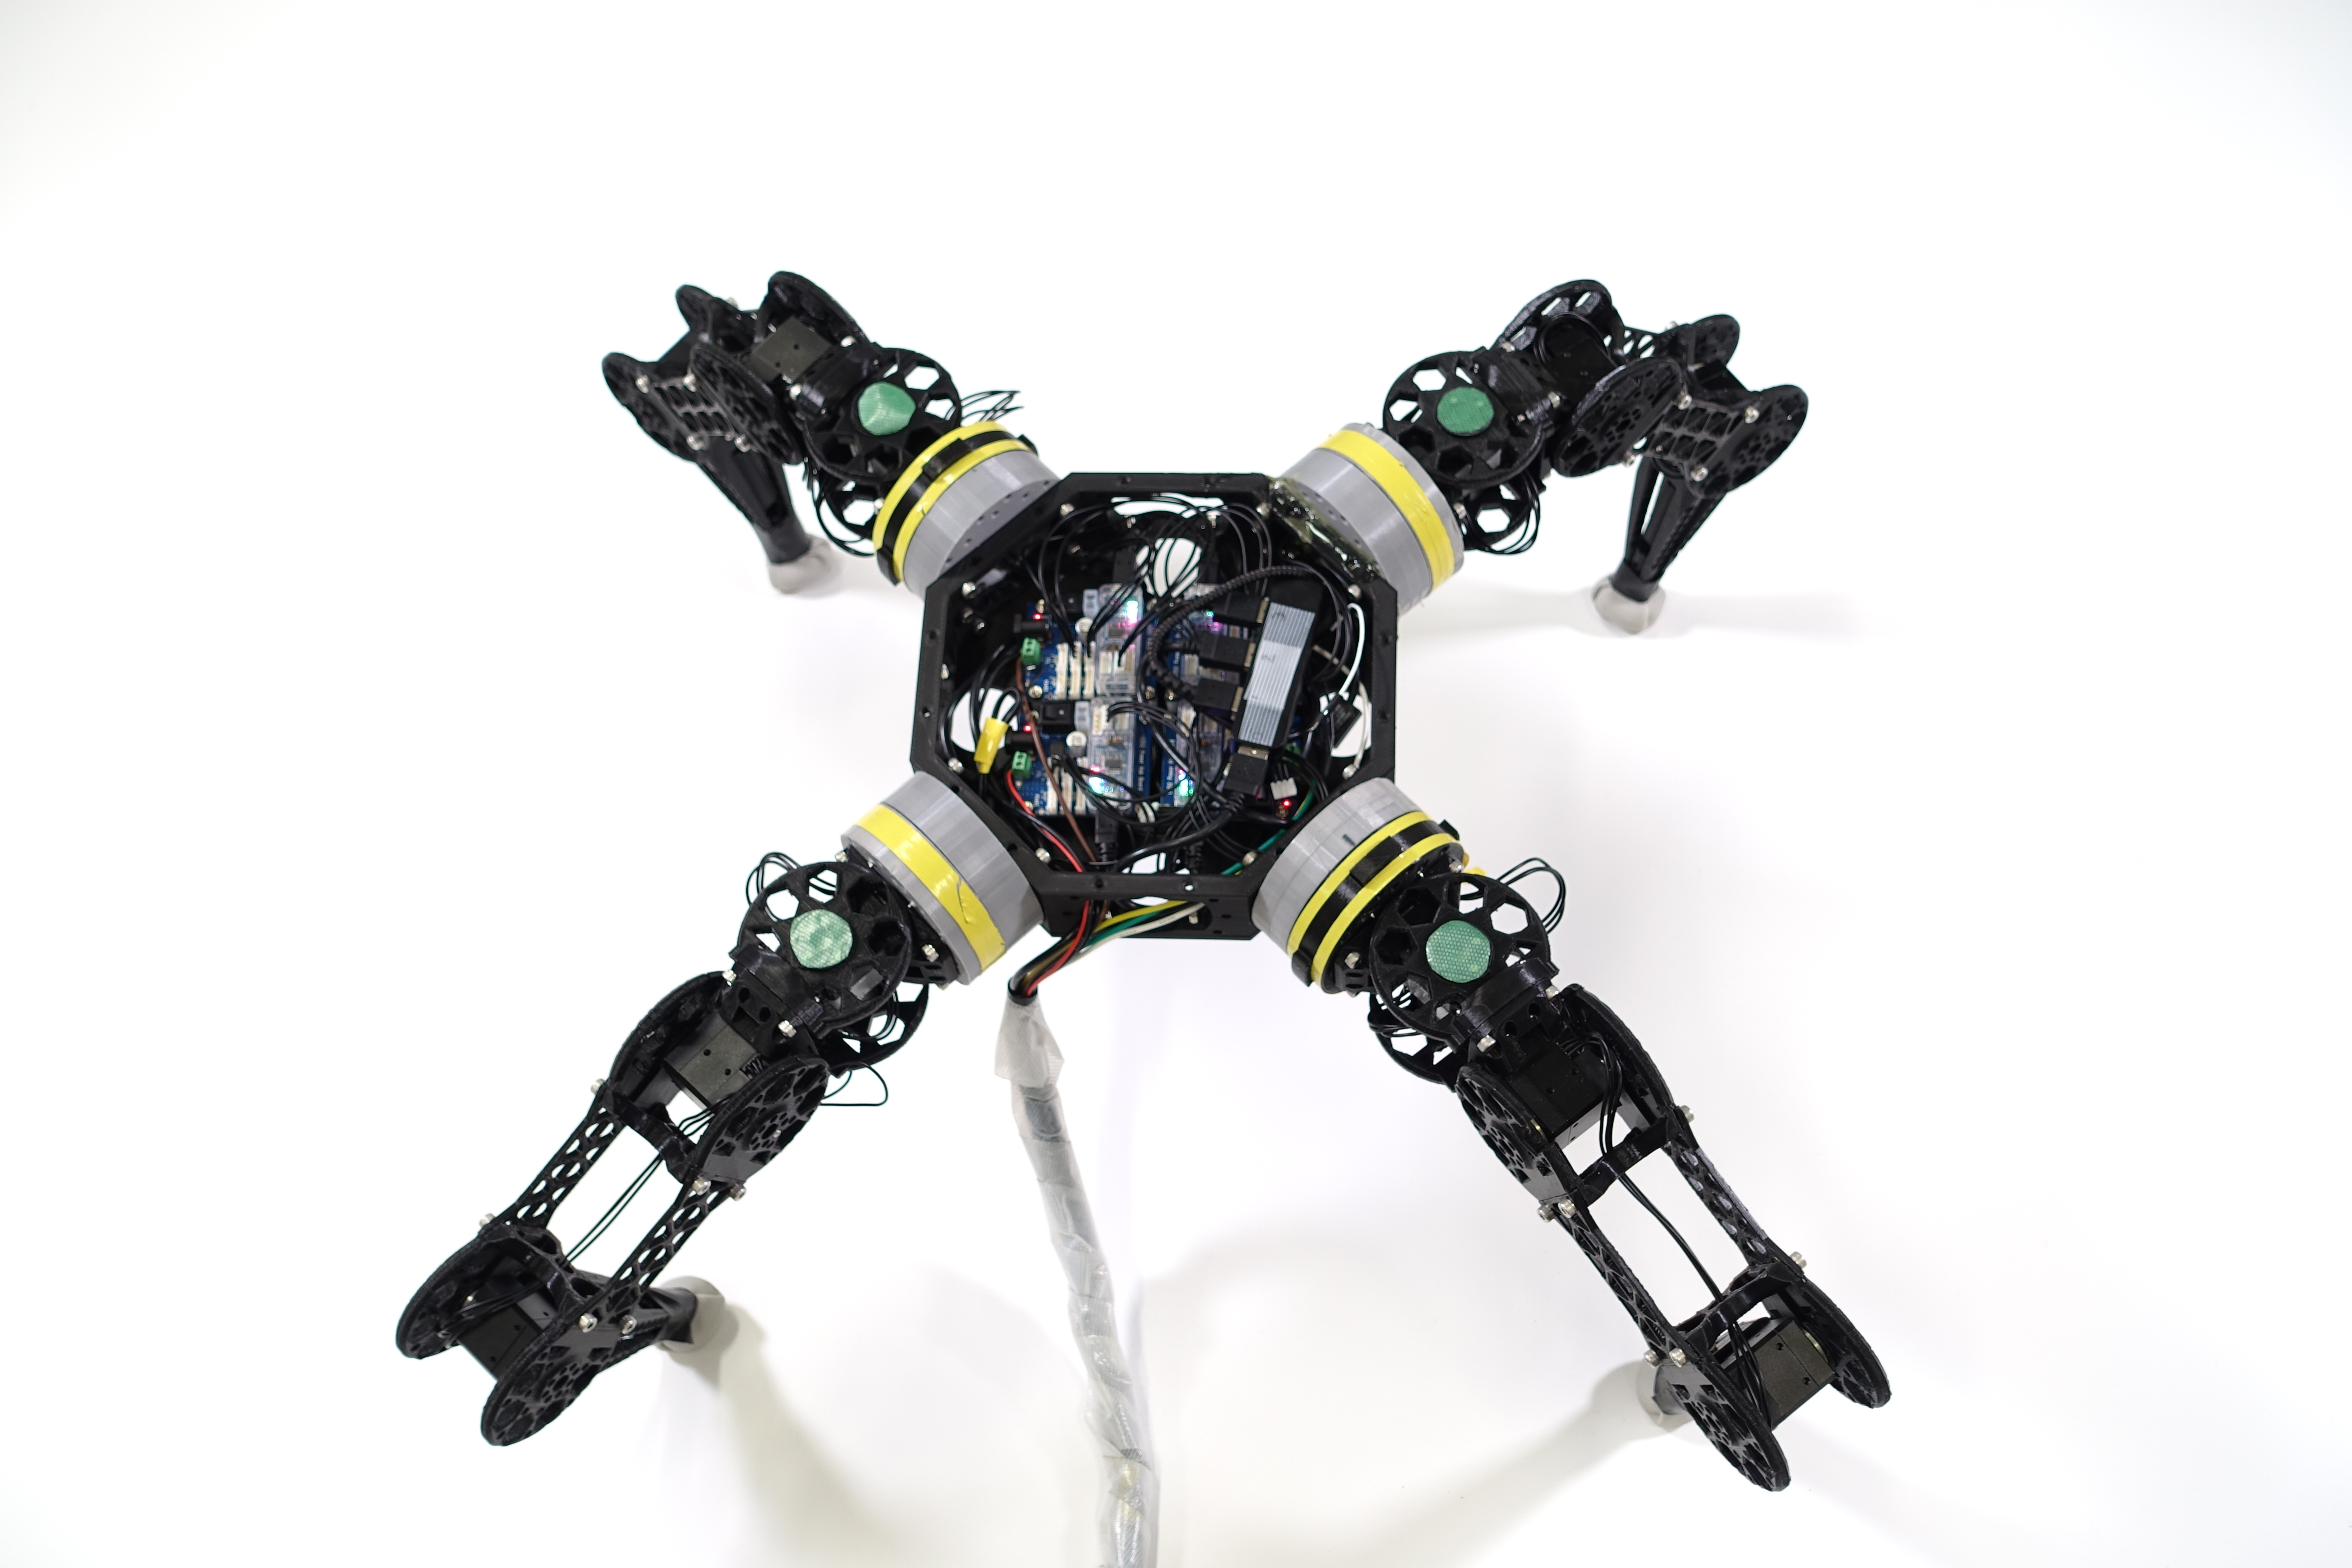
\includegraphics[width=70mm]{./fig/chap4/body_movement/n05pitch.JPG}
        \caption{Body rotates -5 degrees in pitch.}
        \label{nrotpitch}
    \end{subfigure}
    \\
    \begin{subfigure}[b]{0.45\textwidth}
        \centering
        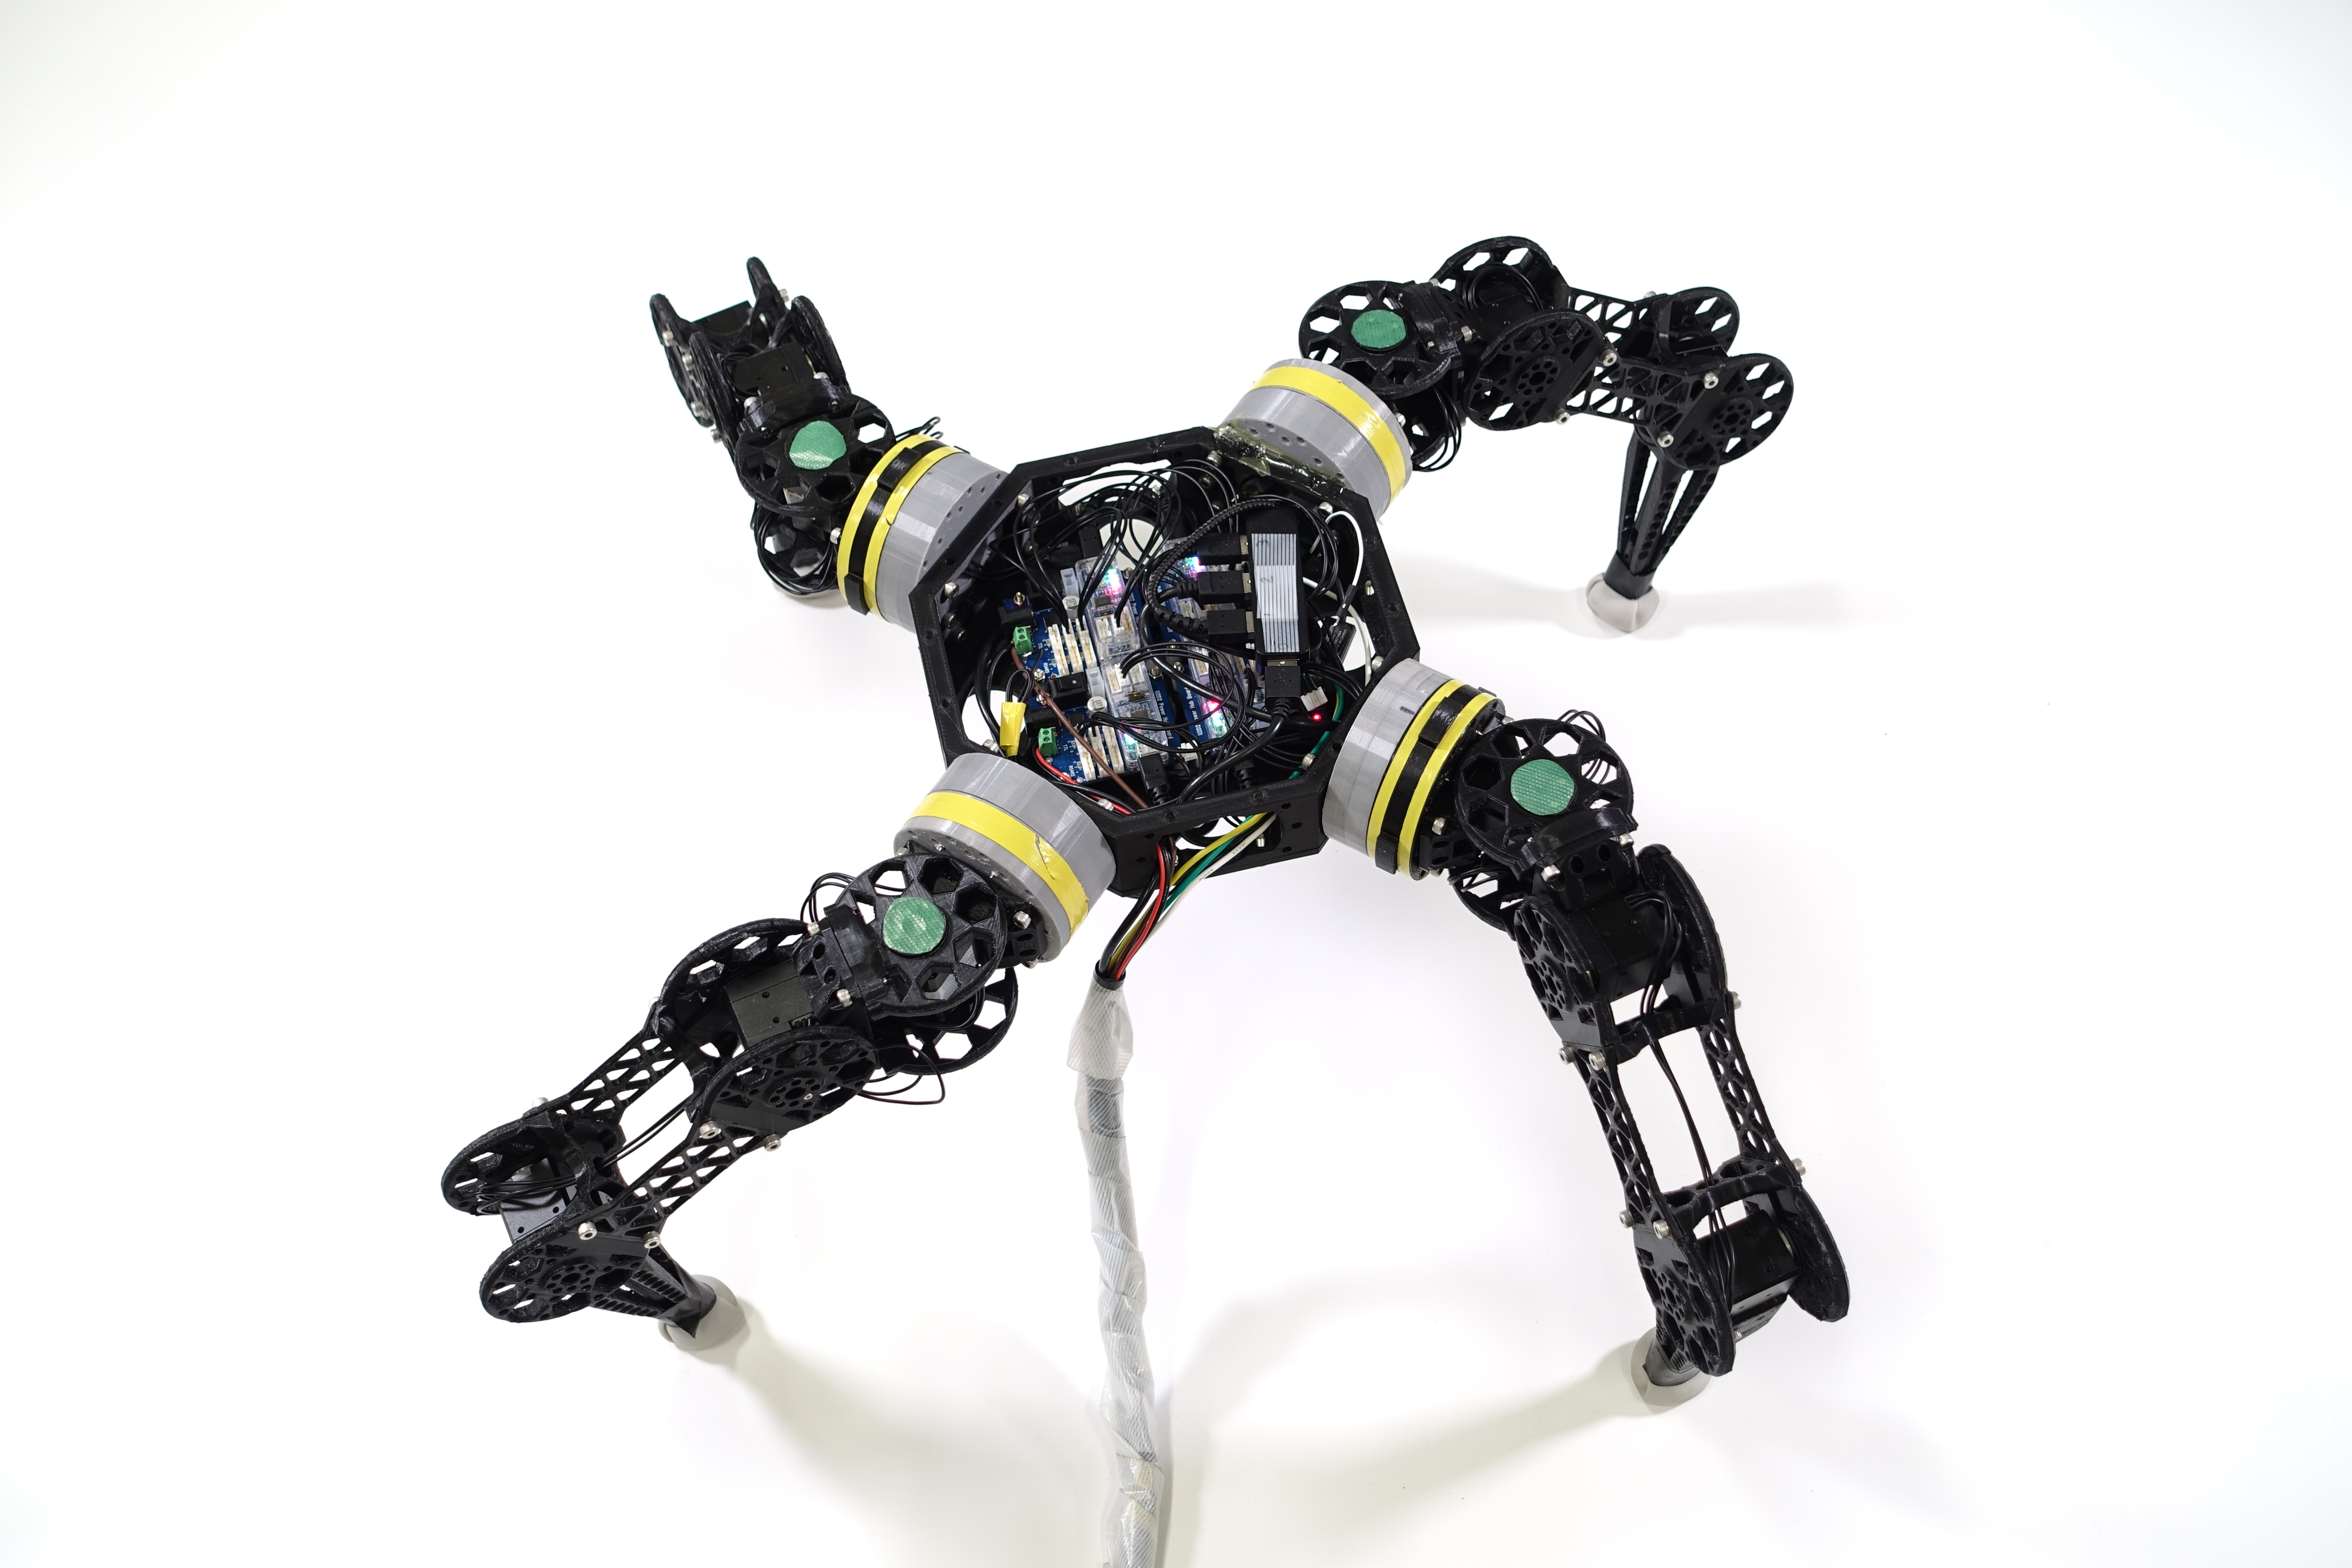
\includegraphics[width=70mm]{./fig/chap4/body_movement/p10yaw.JPG}
        \caption{Body rotates 10 degrees in yaw.}
        \label{protyaw}
    \end{subfigure}
    \begin{subfigure}[b]{0.45\textwidth}
        \centering
        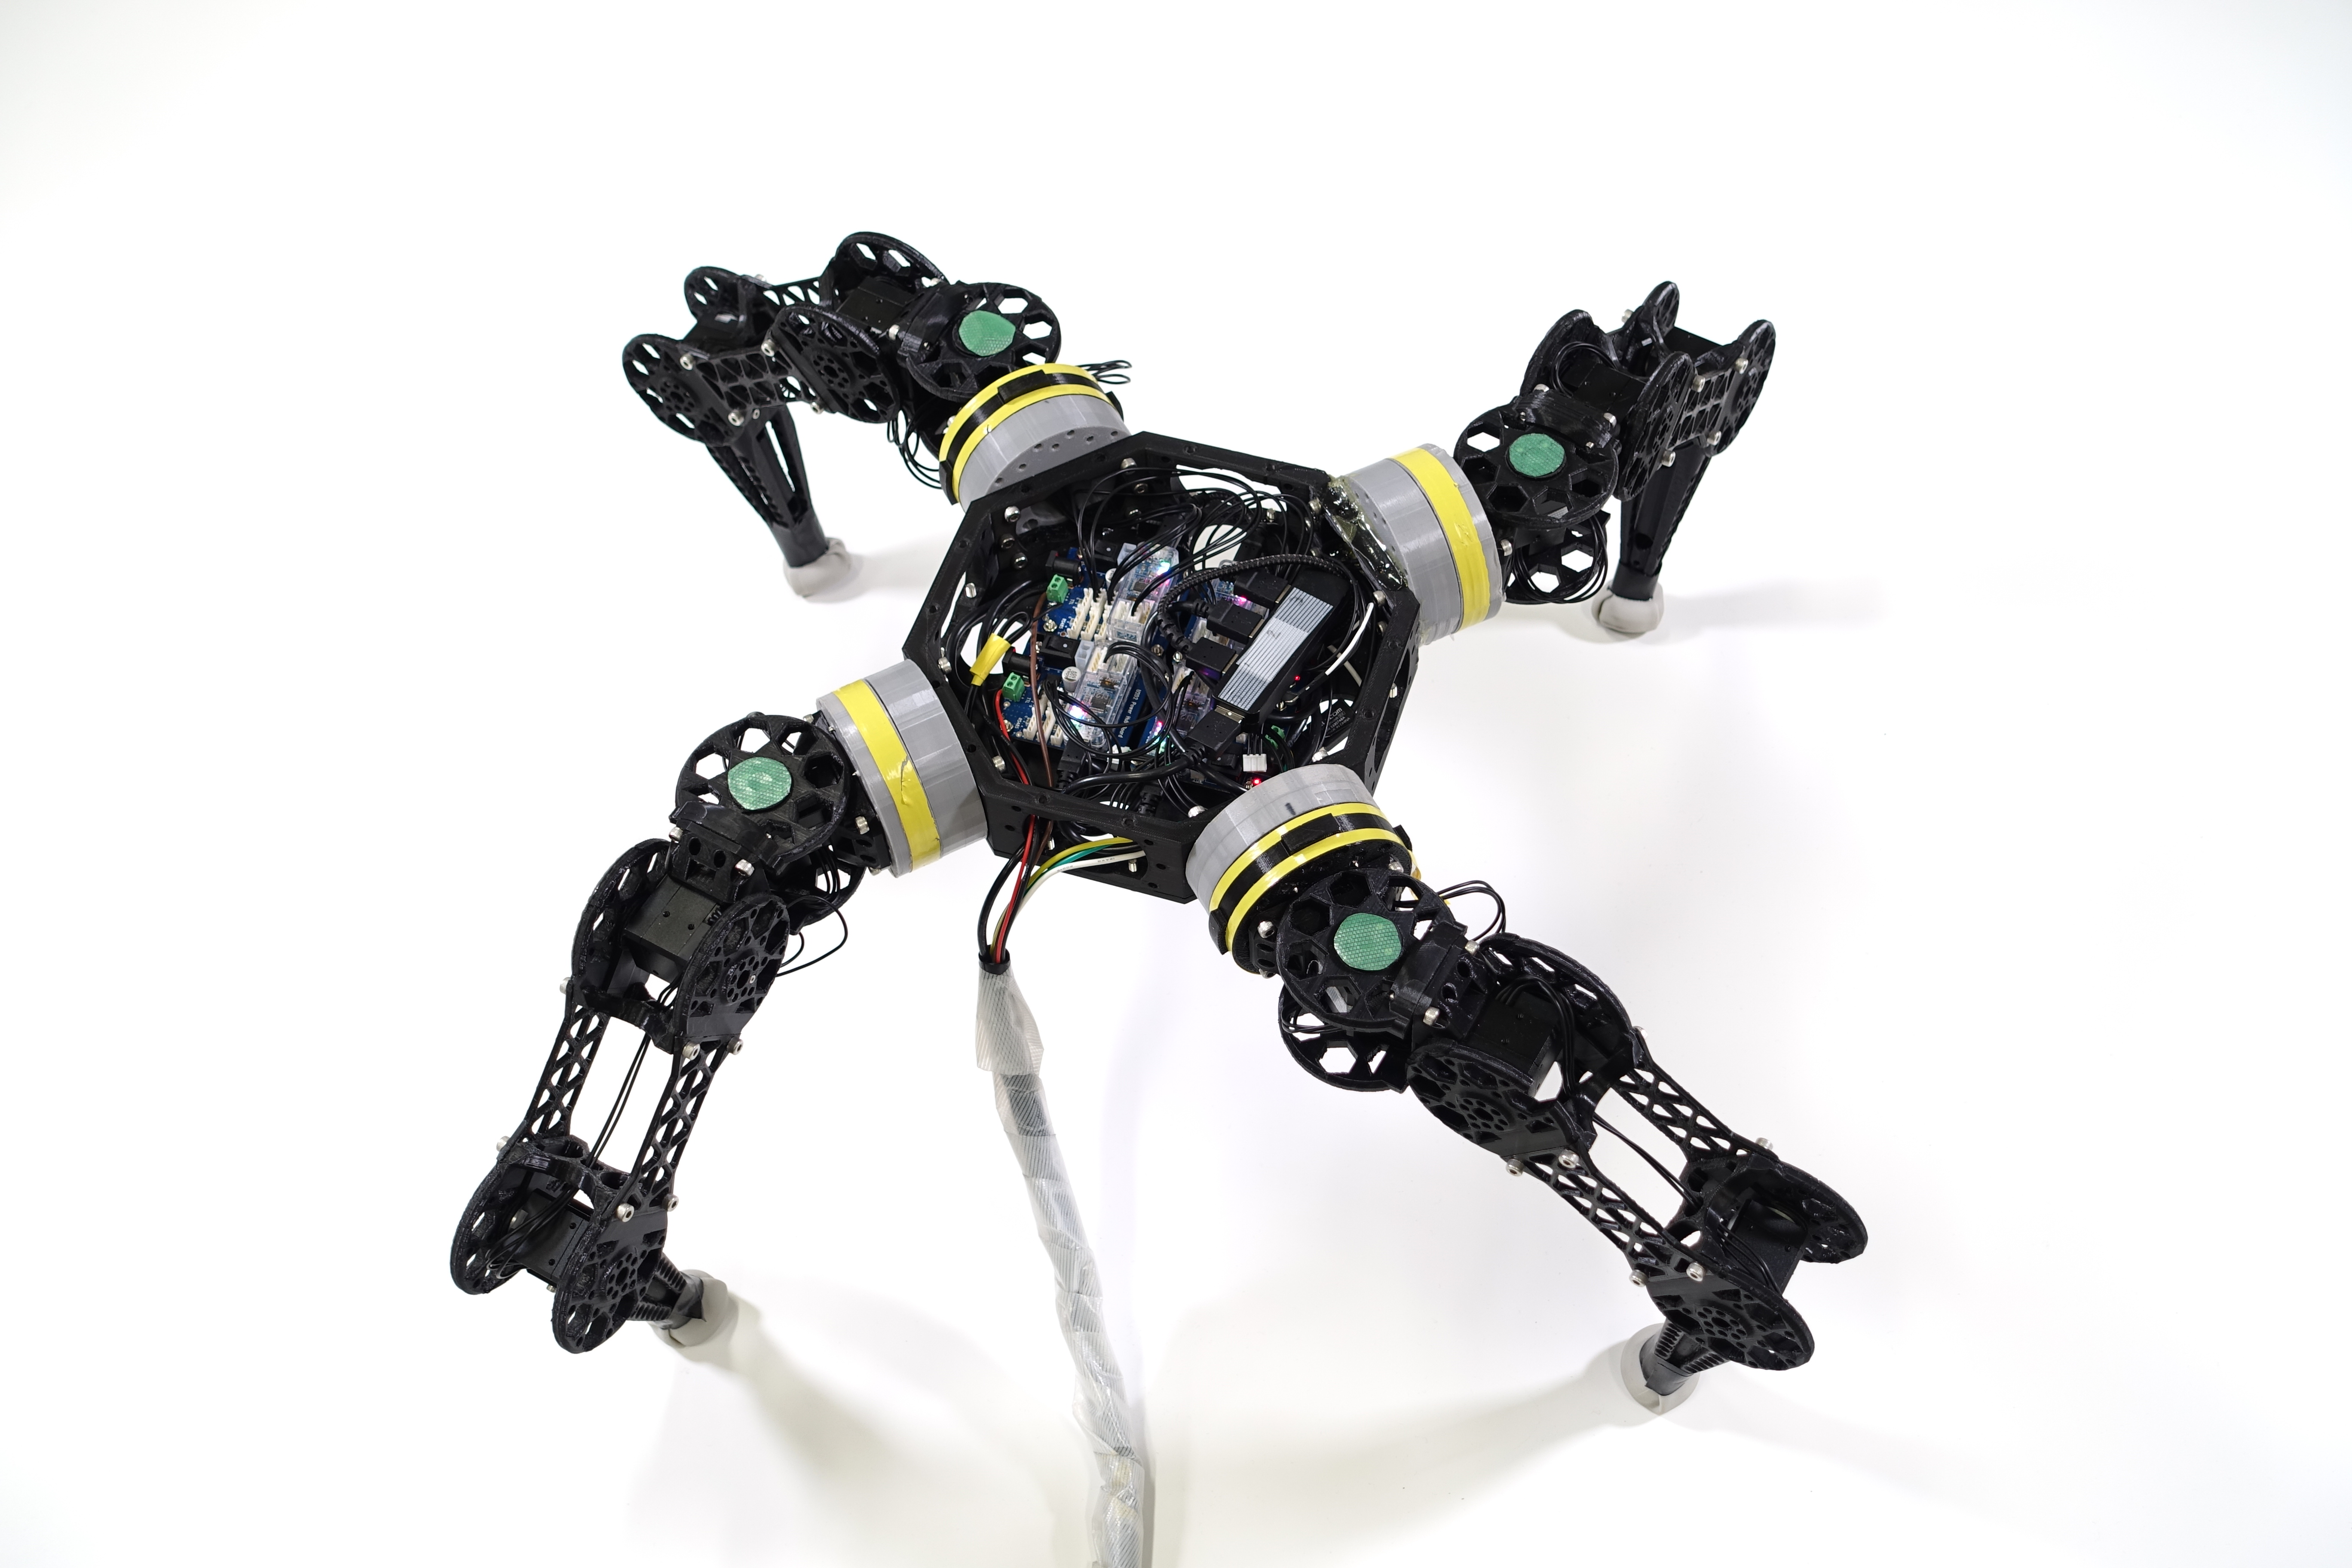
\includegraphics[width=70mm]{./fig/chap4/body_movement/n10yaw.JPG}
        \caption{Body rotates -10 degrees in yaw.}
        \label{nrotyaw}
    \end{subfigure}
    \caption{Body rotational movement.}
    \label{rot}
\end{figure}

\subsection{Gait Generation:}

\begin{enumerate}
    \item \textbf{End-effector Trajectory Generator}
    
\hspace{0.5cm}The trajectory of the legs step is calculated in the gait generator to perform gait patterns and stride vector. Each step along the trajectory involves determining the position of the leg. During the swing phase of each gait pattern, the leg's tip follows a sinusoidal trajectory. By iteratively computing the trajectory for each step, legged robots can generate stable and efficient gaits.

The trajectory equation for each step is given as:

\vspace{2mm}
\begin{equation}
    z(t) = \text{{$S$}} \times \sin\left(\frac{{\pi}}{{\text{{$L$}}}} \times \text{{$t$}}\right)
\end{equation}
\vspace{2mm}

where:
\begin{itemize}
    \item $S$ is step height.
    \item $L$ is step distance.
    \item $t$ is time step.
\end{itemize}

\begin{figure}[h]
  \centering
  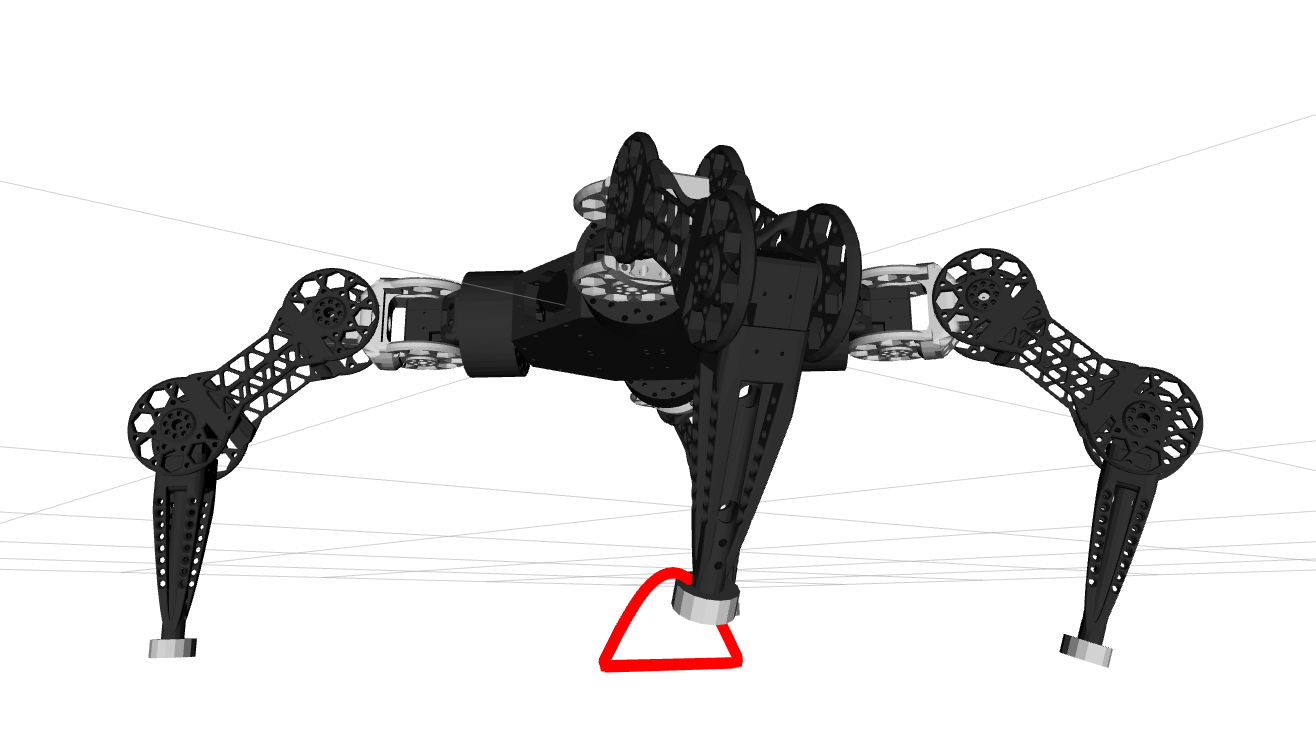
\includegraphics[width=\linewidth]{./fig/chap4/stride/stride1.png}
  \vspace{2mm}
  \caption{Stride generation with sine function.}\label{stride}
\end{figure}

    \item \textbf{Gait Planner}
    
\hspace{0.5cm}With stride vector generation, gait planner plans the swing and stance phases of leg motion, enabling the generation of various gait patterns, including trot and dynamic crawl gait, as shown in Figure \fig{gait_diagram}. The timing of these gait cycles and the desired state of the leg are sent to the end effector's position controller to generate either swing or stance trajectory following the time step of the leg in the gait cycle. The series of snapshots for trot gait and crawl gait are presented in \fig{trotsnap} and \fig{crawlsnap}, respectively.
\end{enumerate}

% \subsection{Gait Generation}
\begin{figure}[t]
  \centering
  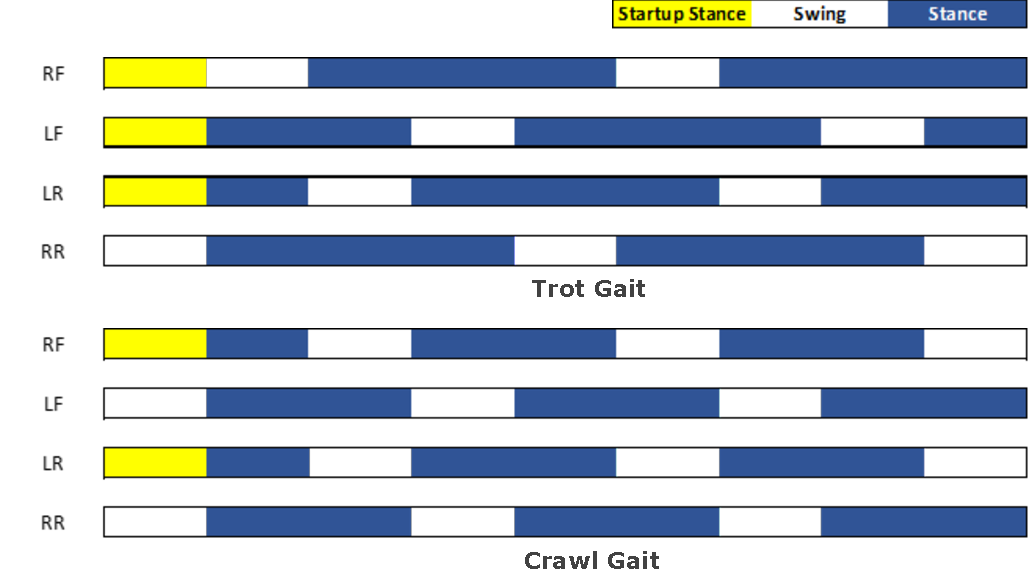
\includegraphics[width=\linewidth]{./fig/locomotion/diagram/gaitdiagram.pdf}
  \vspace{2mm}
  \caption{Gait diagram of walking motion.}\label{gait_diagram}
\end{figure}

\begin{figure}[t]
  \centering
  \begin{minipage}[b]{0.32\textwidth}
    \centering
    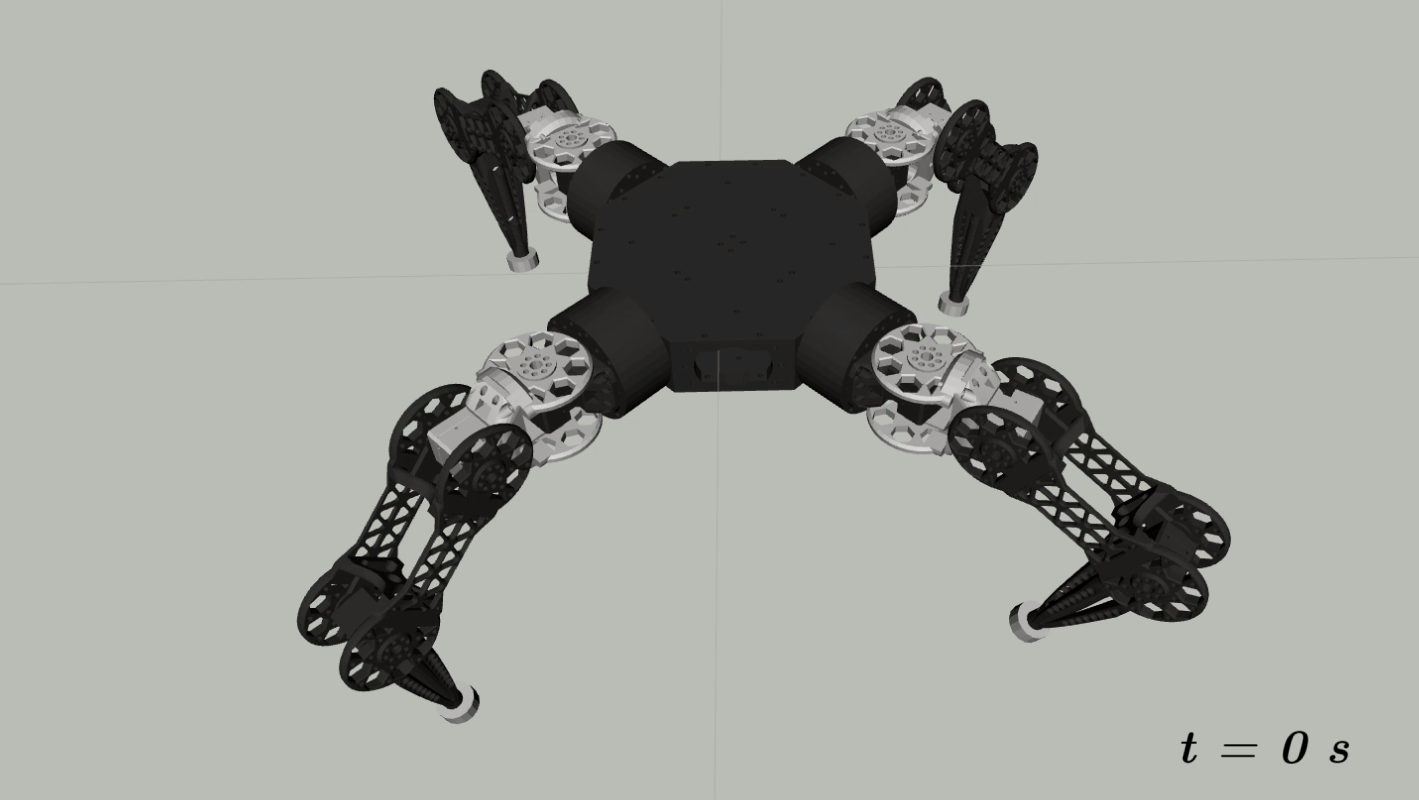
\includegraphics[clip, width=\linewidth]{./fig/chap4/gait/trot/t_step1.png}
  \end{minipage}
  \begin{minipage}[b]{0.32\textwidth}
    \centering
    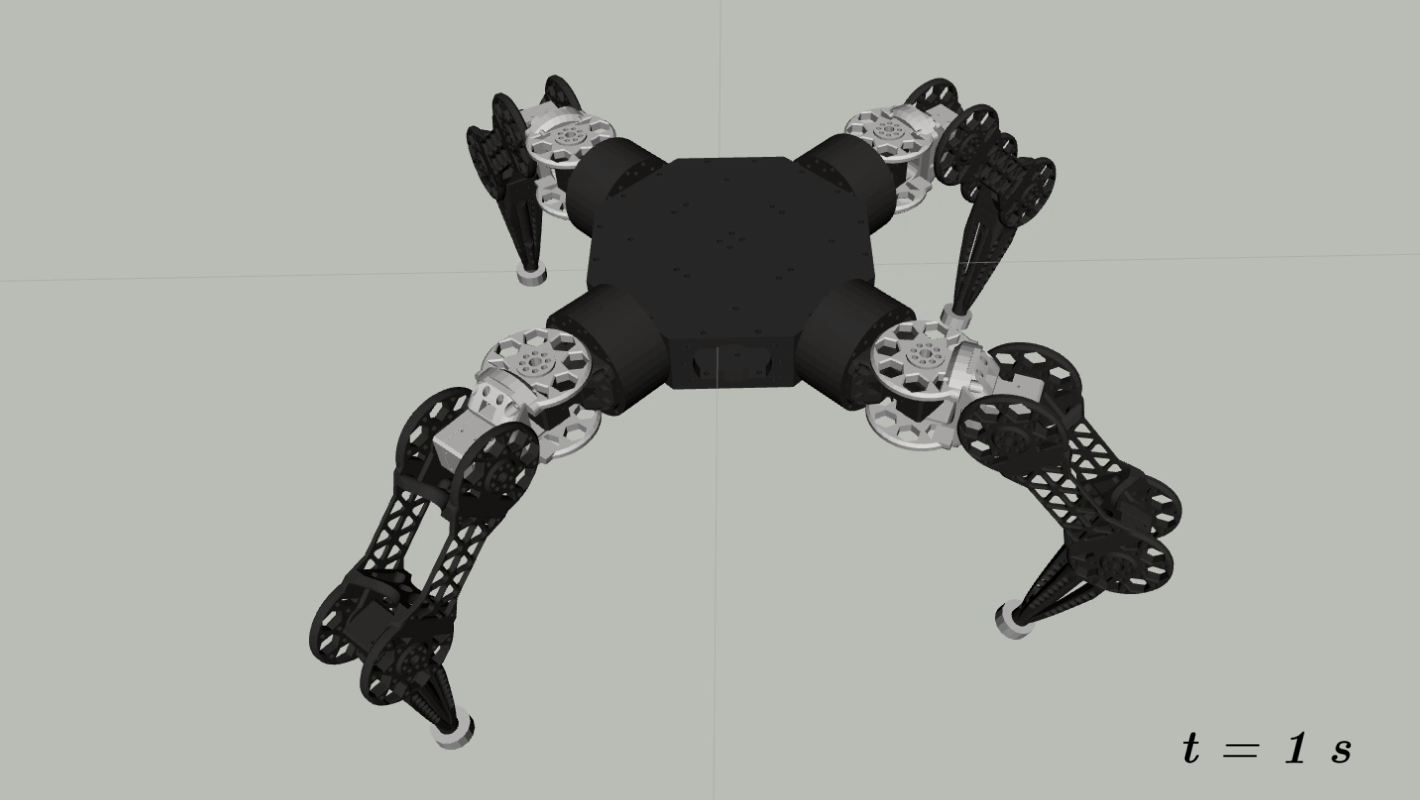
\includegraphics[clip, width=\textwidth]{./fig/chap4/gait/trot/t_step2.png}
  \end{minipage}
  \begin{minipage}[b]{0.32\textwidth}
    \centering
    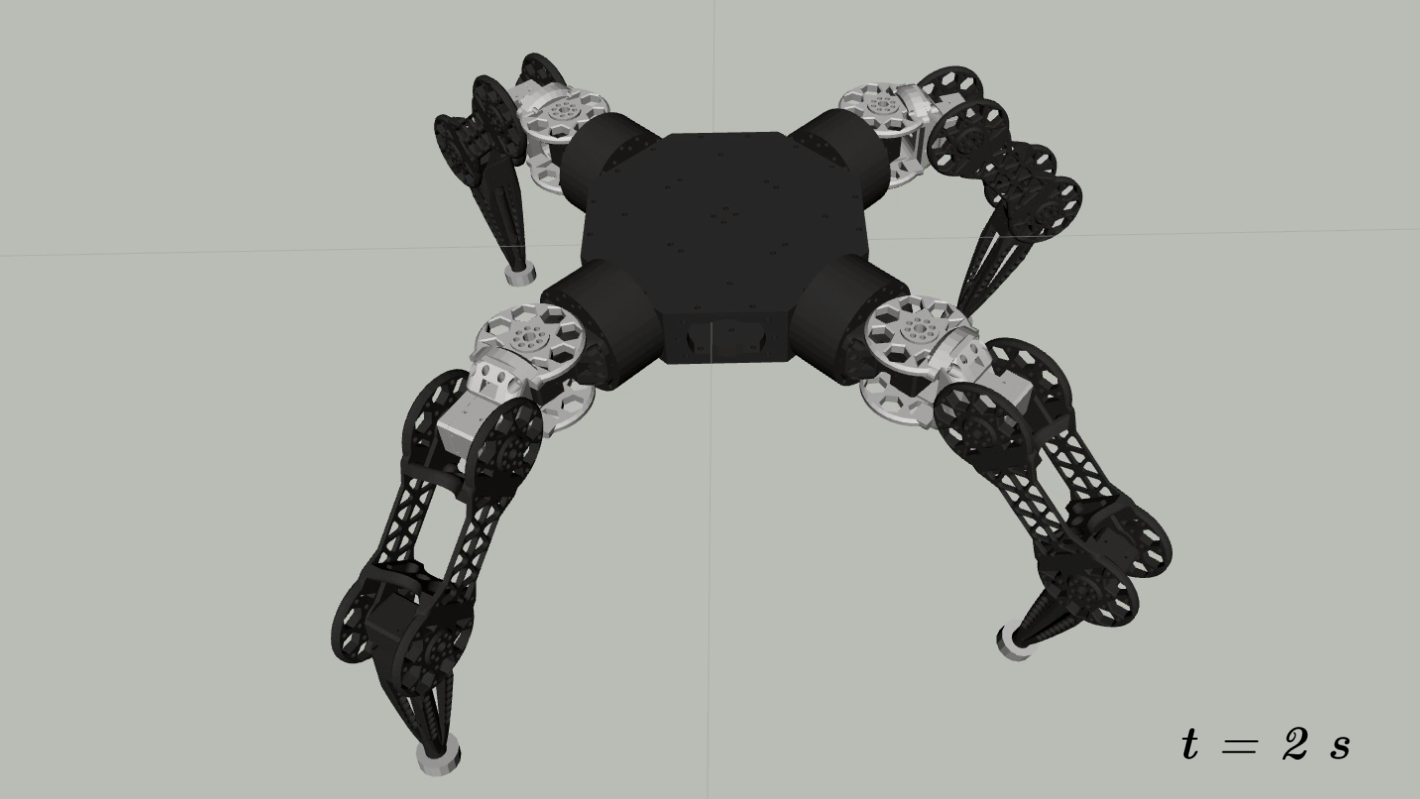
\includegraphics[clip, width=\textwidth]{./fig/chap4/gait/trot/t_step3.png}
  \end{minipage}\\
  \begin{minipage}[b]{0.32\textwidth}
    \centering
    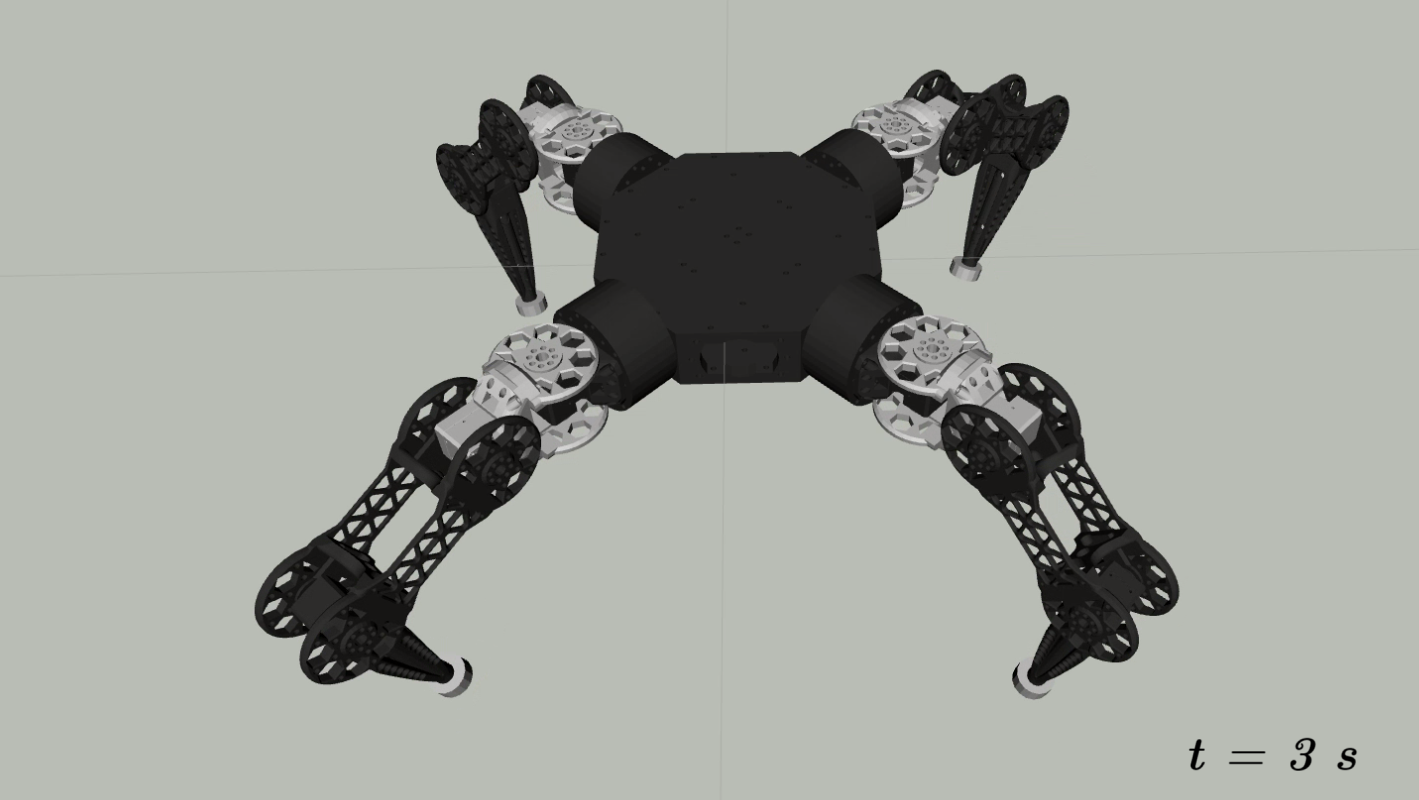
\includegraphics[clip, width=\textwidth]{./fig/chap4/gait/trot/t_step4.png}
  \end{minipage}
  \begin{minipage}[b]{0.32\textwidth}
    \centering
    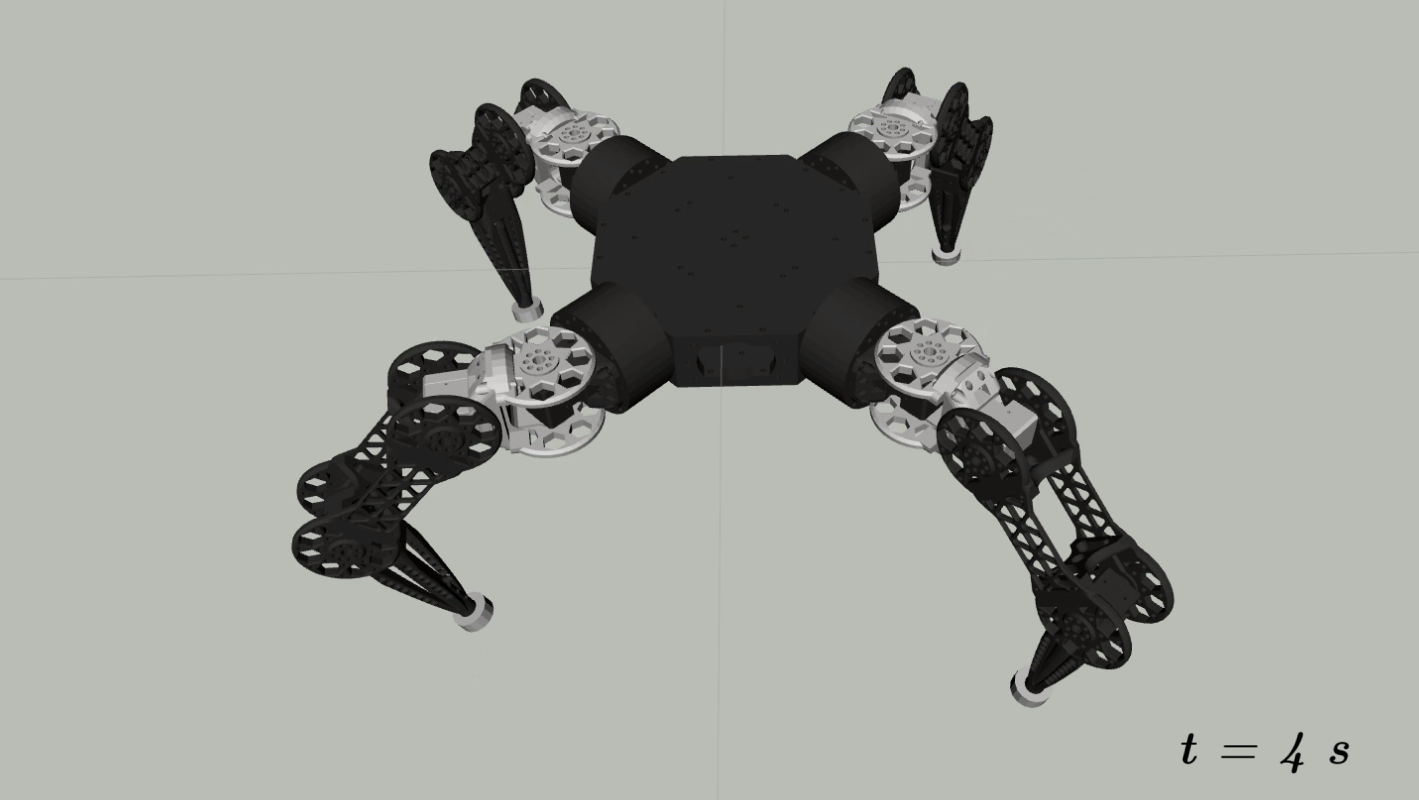
\includegraphics[clip, width=\textwidth]{./fig/chap4/gait/trot/t_step5.png}
  \end{minipage}
  \begin{minipage}[b]{0.32\textwidth}
    \centering
    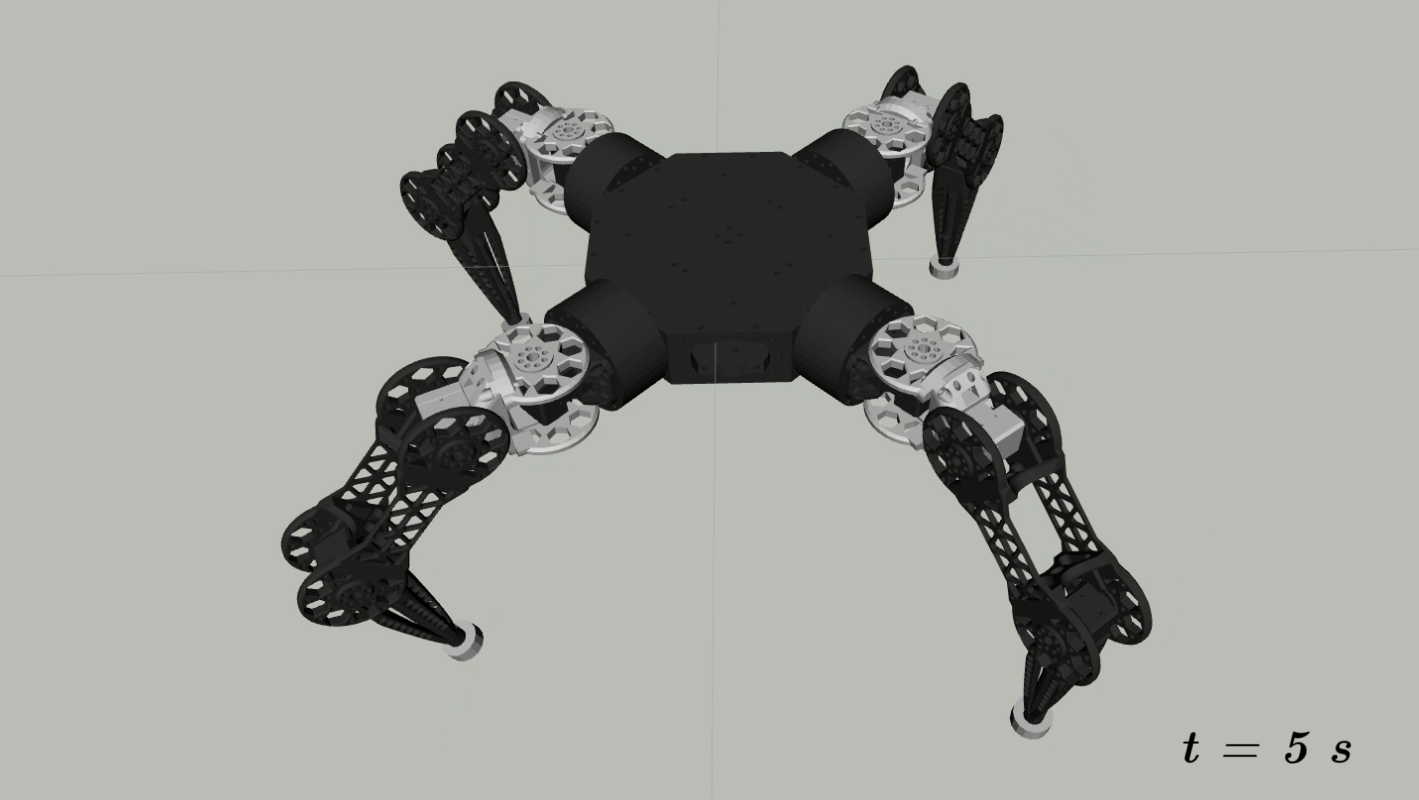
\includegraphics[clip, width=\textwidth]{./fig/chap4/gait/trot/t_step6.png}
  \end{minipage}\\
\caption{Series pictures of Moonbot walking with trot gait towards the top of the page. The pictures were taken every 1 sex from left to right, top to bottom.}
\label{trotsnap}
\end{figure}

\begin{figure}[t]
  \centering
  \begin{minipage}[b]{0.32\textwidth}
    \centering
    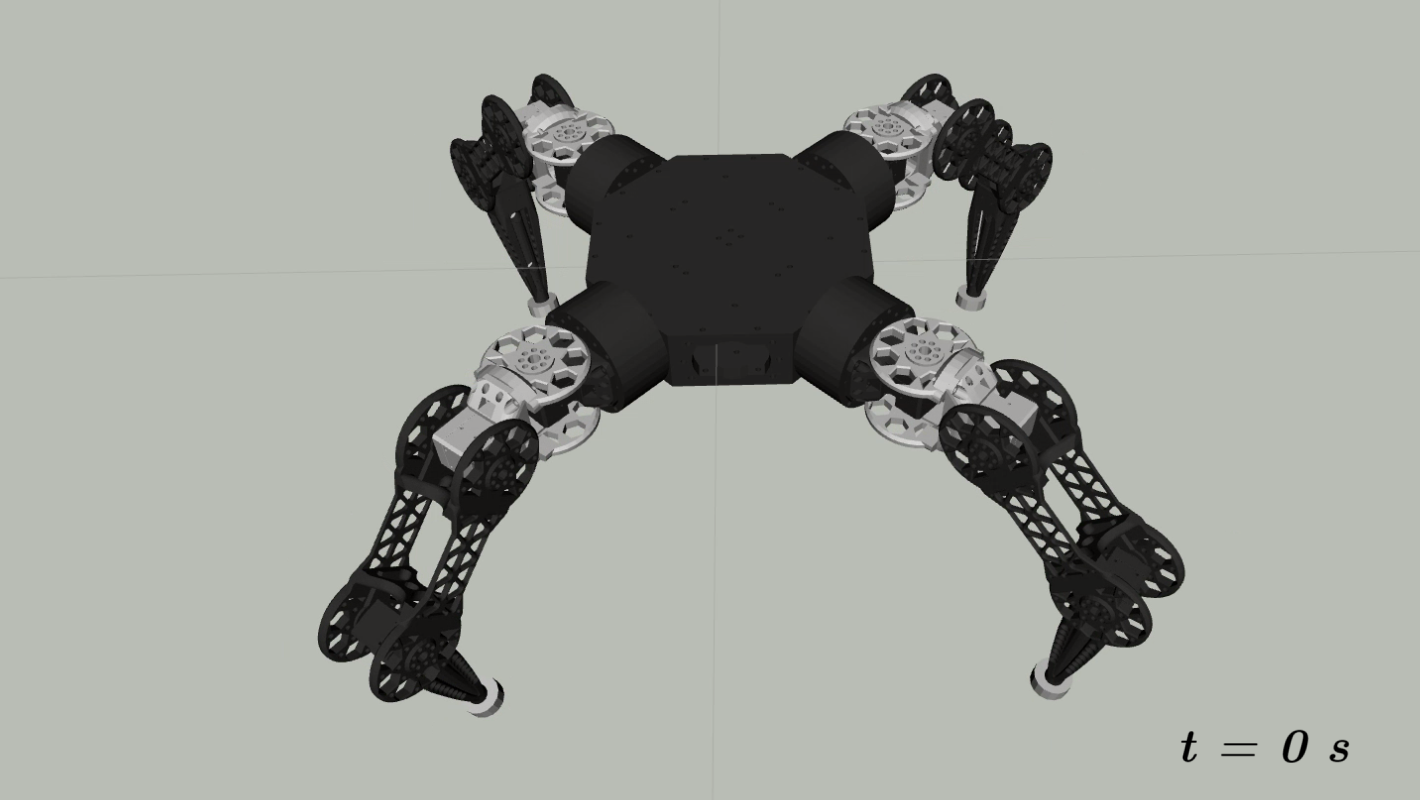
\includegraphics[clip, width=\linewidth]{./fig/chap4/gait/crawl/c_zmp1.png}
  \end{minipage}
  \begin{minipage}[b]{0.32\textwidth}
    \centering
    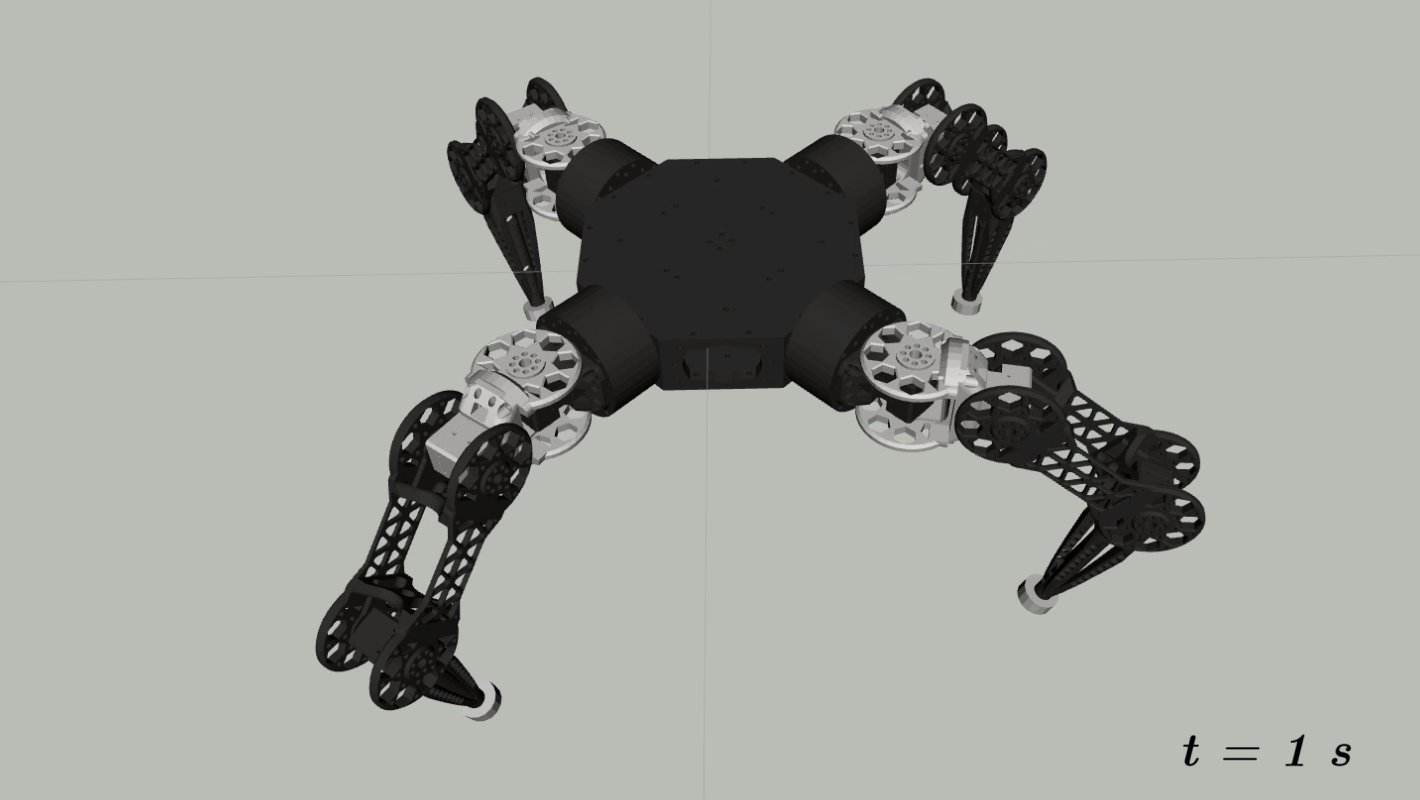
\includegraphics[clip, width=\textwidth]{./fig/chap4/gait/crawl/c_step1.png}
  \end{minipage}
  \begin{minipage}[b]{0.32\textwidth}
    \centering
    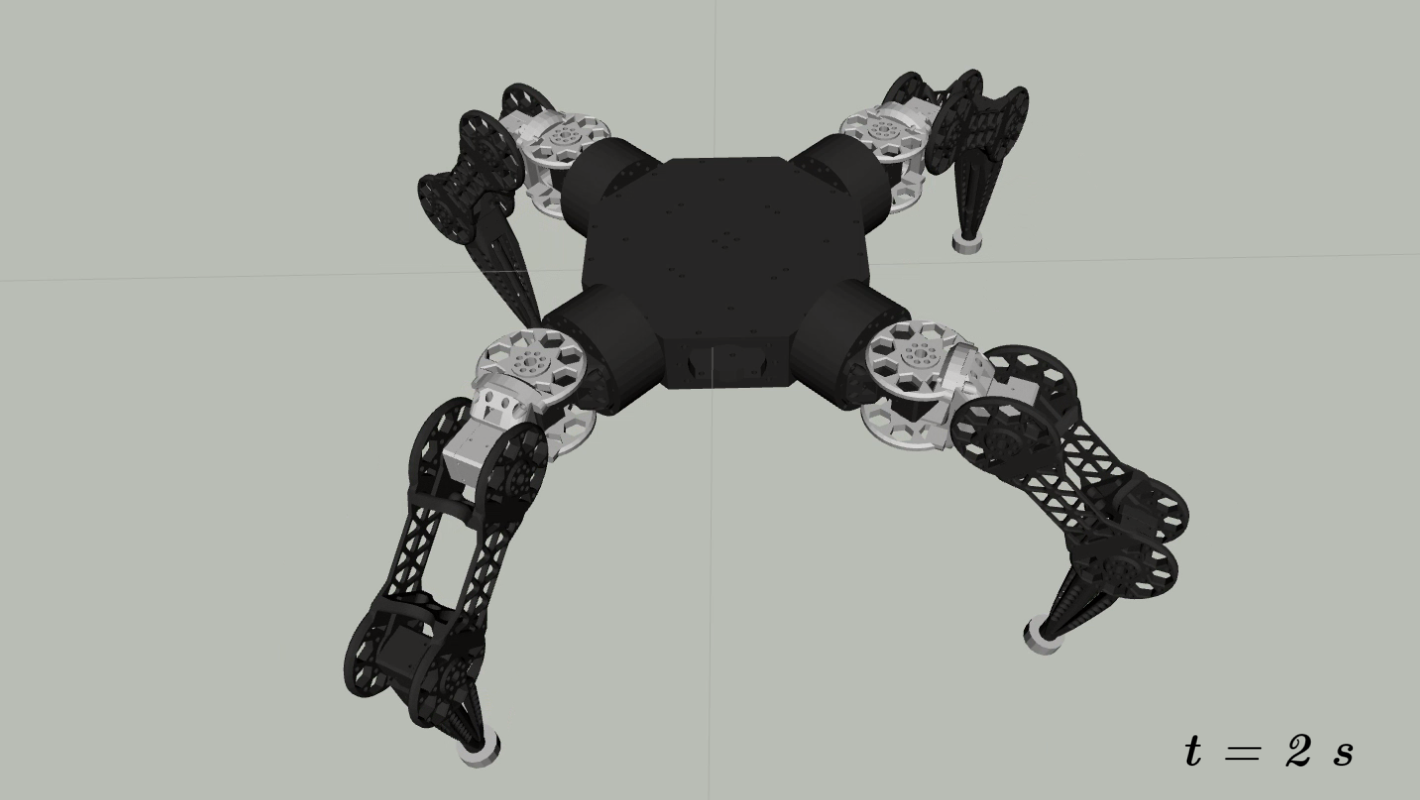
\includegraphics[clip, width=\textwidth]{./fig/chap4/gait/crawl/c_step2.png}
  \end{minipage}\\
  \begin{minipage}[b]{0.32\textwidth}
    \centering
    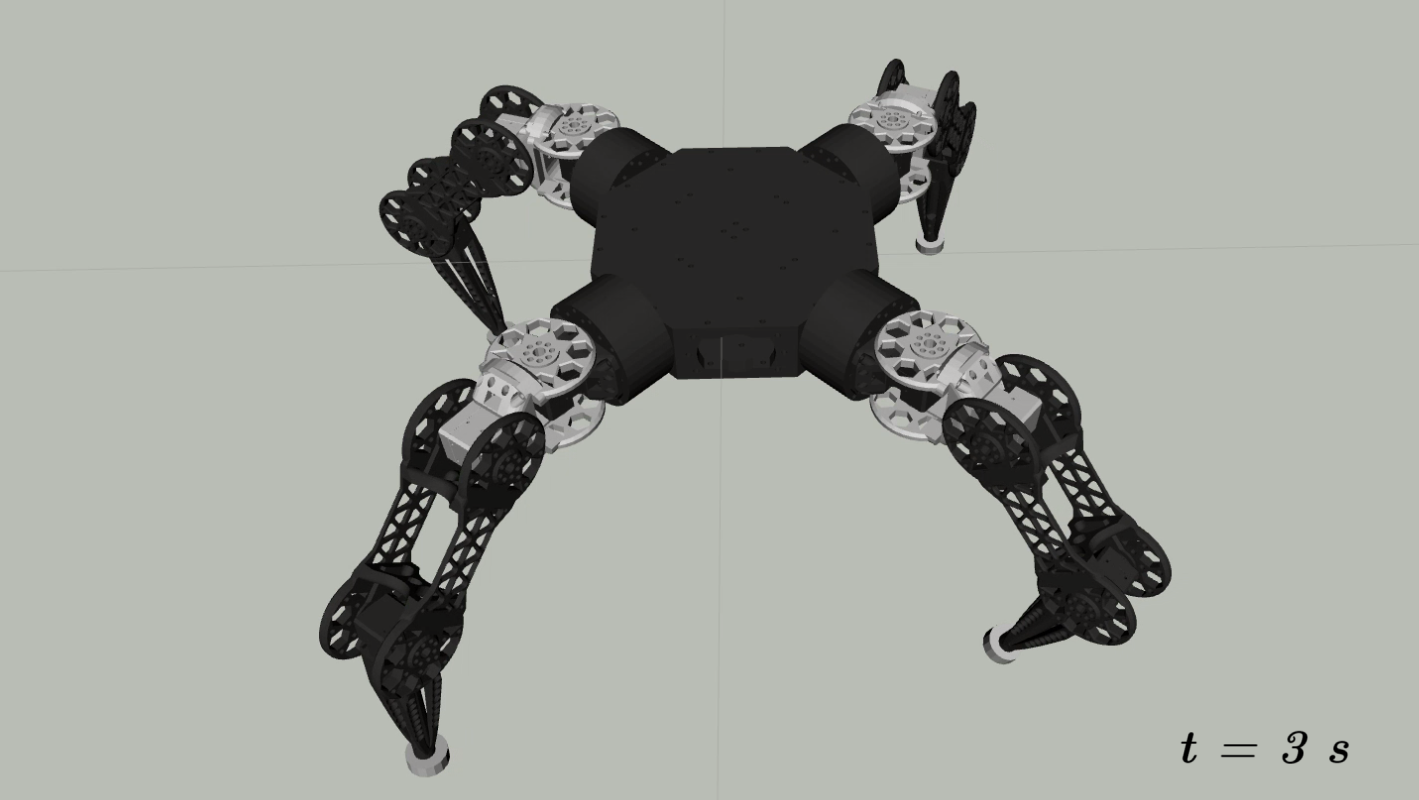
\includegraphics[clip, width=\textwidth]{./fig/chap4/gait/crawl/c_zmp2.png}
  \end{minipage}
  \begin{minipage}[b]{0.32\textwidth}
    \centering
    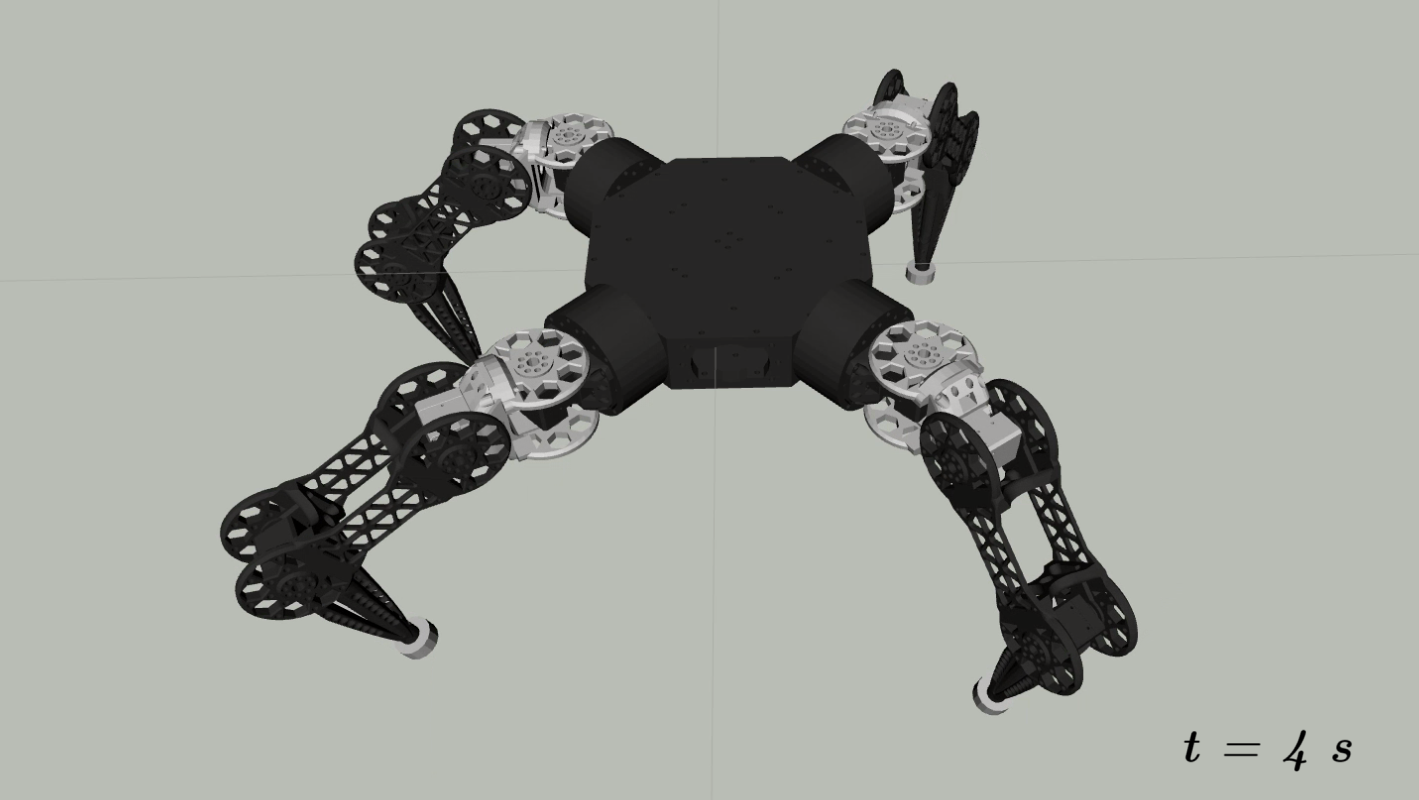
\includegraphics[clip, width=\textwidth]{./fig/chap4/gait/crawl/c_step3.png}
  \end{minipage}
  \begin{minipage}[b]{0.32\textwidth}
    \centering
    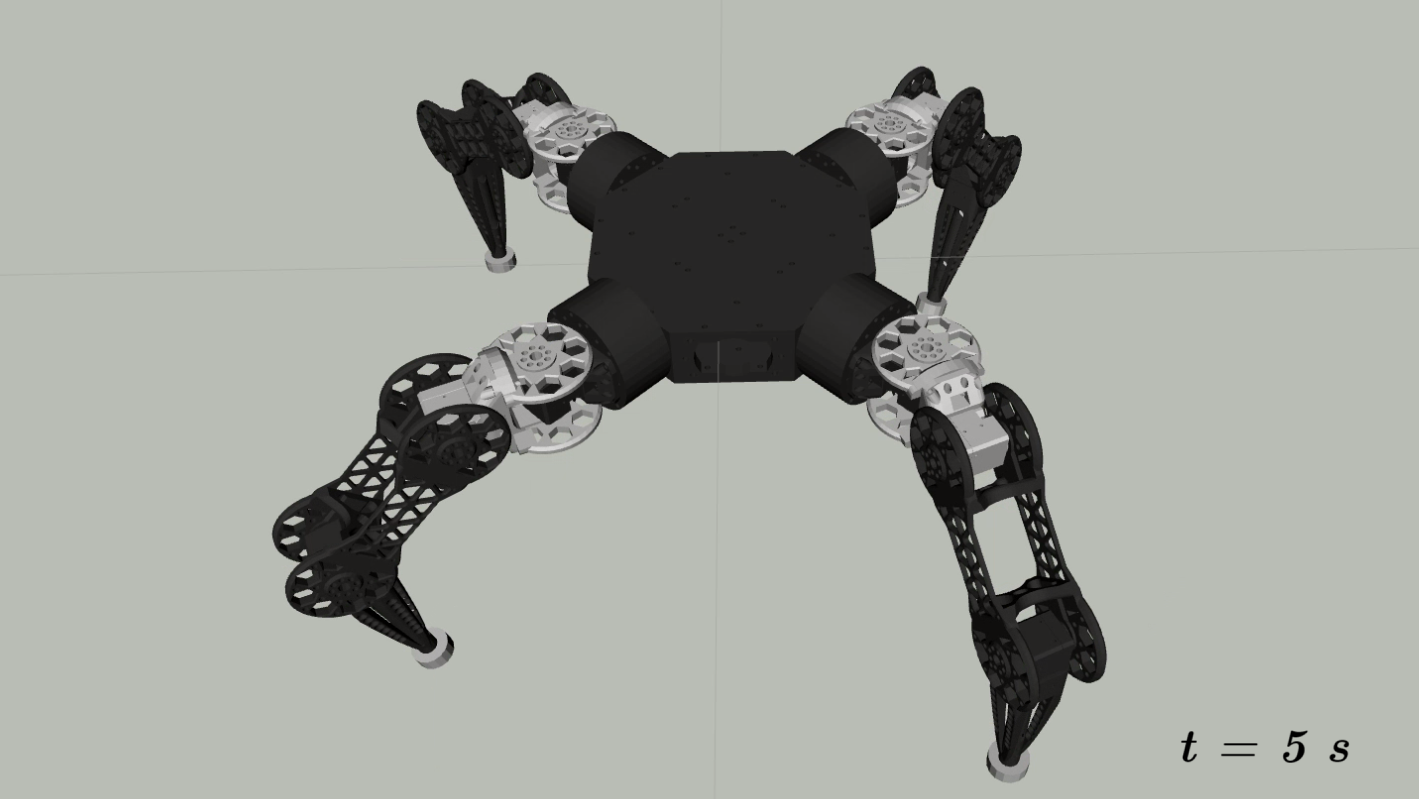
\includegraphics[clip, width=\textwidth]{./fig/chap4/gait/crawl/c_step4.png}
  \end{minipage}\\
\caption{Series pictures of Moonbot walking with crawl gait towards the top of the page. The pictures were taken every 1 sex from left to right, top to bottom.}
\label{crawlsnap}
\end{figure}

%%% EOF %%%